% You should title the file with a .tex extension (hw1.tex, for example)
\documentclass[11pt]{article}

\usepackage{amsmath}
\usepackage{mathtools}
\usepackage{amssymb}
\usepackage{wrapfig}
\usepackage{fancyhdr}
\usepackage{tikz-qtree}
\usepackage{tikz-qtree-compat}
\usepackage[normalem]{ulem}
\usepackage{tikz}
\usepackage{graphicx}
\usepackage{lineno}
\DeclareMathOperator*{\argmin}{argmin}
\DeclareMathOperator*{\argmax}{argmax}

\oddsidemargin0cm
\topmargin-2cm     %I recommend adding these three lines to increase the 
\textwidth16.5cm   %amount of usable space on the page (and save trees)
\textheight23.5cm  

\newcommand{\question}[2] {\vspace{.25in} \hrule\vspace{0.5em}
\noindent{\bf #1: #2} \vspace{0.5em}
\hrule \vspace{.10in}}
\renewcommand{\part}[1] {\vspace{.10in} {\bf (#1)}}
\linespread{1.5}

\newcommand{\myname}{Anonymous Authors}
\newcommand{\myhwnum}{12}

\setlength{\parindent}{0pt}
\setlength{\parskip}{5pt plus 1pt}
 
\DeclarePairedDelimiter\abs{\lvert}{\rvert}%

\pagestyle{fancyplain}

\begin{document}
\medskip                        % Skip a "medium" amount of space
                                % (latex determines what medium is)
                                % Also try: \bigskip, \littleskip

\thispagestyle{plain}
{\Large Interrogating theoretical models of neural computation with deep learning} \\
Sean R. Bittner, Agostina Palmigiano, Alex T. Piet, Chunyu A. Duan, Francesca Mastrogiuseppe, Srdjan Ostojic, Carlos D. Brody, Kenneth D. Miller, and John P. Cunningham.

\linenumbers
\section{Abstract}
The cornerstone of theoretical neuroscience is the circuit model: a system of equations that captures a hypothesized neural mechanism of scientific importance.  
At its best, such a model will give rise to an experimentally observed phenomenon -- whether behavioral or in terms of neural activity -- and thus can offer insight into neural computation.  
The operation of these circuits, like all models, critically depends on the choices of model parameters.  
Historically, the gold standard has been to analytically derive the relationship between model parameters and computational properties.  
However, this enterprise quickly becomes infeasible as biologically realistic constraints are included into the model, resulting often in \emph{ad hoc} approaches to understanding the relationship between model and computation.  
We bring cutting edge machine learning -- the use of deep learning for probabilistic inference -- to bear on this problem, learning distributions of parameters that produce the specified properties of computation.   
Importantly, the techniques we introduce offer a logical and unbiased means to understand the implications of model parameter choices on computational properties of interest.  
We use these techniques to produce a novel characterization of sensitivity in the stomatogastric ganglion, insights into neuron-type input-responsivity in primary visual cortex, new understanding of rapid task switching in superior colliculus models, and improved attribution of bias in a low-rank recurrent neural network model. 
More generally, this work moves us away from the tradeoff of biological realism vs analytical tractability, and towards the use of modern machine learning for sophisticated interrogation of biologically relevant models.
%(150 word limit) we can ignore that for now up to about 50% \\

\section{Introduction}

The fundamental practice of theoretical neuroscience is to use a mathematical \emph{model} to understand neural computation, whether that computation enables perception, action, or some intermediate processing \cite{abbott2008theoretical}.  
In this field, a neural computation is systematized with a set of equations -- the model -- and these equations are motivated by biophysics, neurophysiology, and other conceptual considerations.
The function of this system is governed by the choice of model parameters, which when configured in some special way, give rise to some measurable signature of a computation.   
The work of analyzing a model then becomes the inverse problem: given a computation of interest, how can we reason about these special parameter configurations -- their likely values, their uniquenesses and degeneracies, their attractor states and phase transitions, and more?  

Consider the idealized practice: a theorist considers a model carefully and analytically derives how model parameters govern the computation.  
Seminal examples of this gold standard include our field's understanding of memory capacity in associative neural networks \cite{hopfield1984neurons}, chaos and autocorrelation timescales in random neural networks \cite{sompolinsky1988chaos}, and the paradoxical effect in excitatory/inhibitory networks \cite{tsodyks1997paradoxical}.  
Unfortunately, as circuit models include more biological realism, theory via analytic derivation becomes intractable.  
This fact creates an unfavorable tradeoff for the theorist.  On the one hand, one may tractably analyze systems of equations with unrealistic assumptions (for example symmetry or gaussianity), producing accurate inferences about parameters of a too-simple model.  On the other hand, one may choose a more biologically relevant model at the cost of \emph{ad hoc} approaches to analysis (simply examining simulated activity), producing questionable or partial inferences about parameters of an appropriately complex, scientifically interesting model.  % intentionally belaboring the "inference about model parameters" to set the mindset of what *the* important question is.

% now transition to ML...
Of course, this same tradeoff has been confronted in many scientific fields characterized by the need to do inference in complex models.  
Notably, the machine learning community has made remarkable progress in recent years, via the use of deep neural networks as a powerful inference engine: a flexible function family that can map observed phenomena (in this case the measurable signal of some computation) back to probability distributions quantifying the likely parameter configurations.  
One celebrated example of this approach from the machine learning community, from which we draw key inspiration for this work, is the variational autoencoder \cite{kingma2013auto, rezende2015variational, not this one; cite the rezende and mohamed vae one from 2013}, which uses a deep neural network to induce an (approximate) posterior distribution on hidden variables in a latent variable model, given data. 
Indeed, these tools have been used to great success in neuroscience as well, in particular for interrogating parameters (sometimes treated as hidden states) in models of both cortical population activity \cite{gao2016linear, zhao2017recursive, barello2018sparse, pandarinath2018inferring} and animal behavior \cite{wiltschko2015mapping, johnson2016composing, batty2019behavenet}. 
These works have used deep neural networks to expand the expressivity and accuracy of statistical models of neural data \cite{paninski2018neural}. 

However, these inference tools have not significantly influenced the study of theoretical neuroscience models, for at least three reasons.  
First, at a practical level, the nonlinearities and dynamics of many theoretical models are such that conventional inference tools (for example mean field blah blah \cite{???}) typically produce a narrow set of insights into these models.  
Indeed, only in the last few years has the deep learning toolkit expanded to a point of relevance to this class of problem.
Second, the object of interest from a theoretical model is not typically data itself, but rather a qualitative phenomenon -- inspection of model behavior, or better, a measurable signature of some computation -- an \emph{emergent property} of the model.  
Third, because theoreticians work carefully to construct a model that has biological relevance, such a model as a result often does not fit cleanly into the framing of a statistical model.  
Technically, because many such models stipulate a noisy system of differential equations that can only be sampled or realized through forward simulation, they lack the explicit likelihood and priors central to the probabilistic modeling toolkit.  

% now we've constructed the tension that theory models need this and statistical models know how to do this... now connect!
To address these three challenges, we developed an inference methodology -- `emergent property inference' -- which learns a distribution over parameter configurations in a theoretical model.  Critically, this distribution is such that draws from the distribution (parameter configurations) correspond to systems of equations that give rise to a specified emergent property.  
First, we stipulate a deep neural network that induces a flexible family of probability distributions over model parameterizations.   We will insist on being able to quantify the probability of various model parameter configurations, and thus we choose the deep neural network to be of the (bijective) normalizing flow class \cite{rezende2015variational}.
Second, we quantify the notion of emergent properties as a set of moment constraints on datasets generated by the model.  
Thus an emergent property is not a single data realization, but a phenomenon or a feature of the model, which is the central object of interest to the theorist (unlike say the statistical neuroscientist).  
The requirement to condition on an emergent property requires the adaptation of deep probabilistic inference methods, and we extend recent tools to do so \cite{loaiza2017maximum}.
Third,  because we can not assume the theoretical model has explicit likelihood on data or the emergent property of interest, we use stochastic gradient techniques in the spirit of likelihood free variational inference \cite{tran2017hierarchical}.    
Taken together, emergent property inference (EPI) provides a methodology for inferring and then reasoning about parameter configurations that give rise to particular emergent phenomena in theoretical models.   
Emergent property inference is described schematically in Fig 1A.

Equipped with this methodology, we investigated four models of historical and current importance in theoretical neuroscience.
These models were chosen to demonstrate generality through ranges of biological realism (conductance-based biophysics to recurrent neural networks), neural system function (pattern generation to abstract cognitive function), and network scale (four to infinite neurons).
First, to clarify the contribution of emergent property inference, we investigate network syncing in a classic model of the stomatogastric ganglion \cite{gutierrez2013multiple}.  
EPI provides a novel insight into how the parameterization of this model can be adjusted with minimal (or maximal) effect to the emergent property of network syncing.   
Second, we display the expanded perspective ["display the expanded perspective" is vacuous] afforded by EPI compared to available analytic techniques by studying input-responsivity in a four neuron-type dynamical model of primary visual cortex.  
Third, we demonstrate how the systematic application of EPI to levels of behavioral accuracy can generate experimentally testable hypotheses regarding connectivity in superior colliculus.  
Fourth, we leverage the flexibility of EPI to uncover the sources of bias in a low-rank recurrent neural network executing Bayesian inference.  
The novel scientific insights offered by EPI contextualize and clarify the previous studies exploring these models and more generally offer a quantitative grounding for theoretical models  going forward, pointing a way to how rigorous statistical inference can enhance theoretical neuroscience at large.

%-------------------

%These works build on a long line of successful research in neural data analysis over the last twenty years \cite{kass2001spike, brown1998statistical, paninski2004maximum, byron2009gaussian, latimer2015single, duncker2019learning} (see review, \cite{paninski2018neural}).  Now, the use of these modern and powerful inference engines has freed researchers from  making model choices as much to accommodate inference, as to represent the computation being studied \cite{gao2015high} (Sorry, I'm confused by which paper PLDS refers to.).

We note that, during our preparation and early presentation of this work \cite{bittnerCOSYNE2019, bittnerBernstein2019}, another work has arisen with broadly similar goals: bringing statistical inference to mechanistic models of neural circuits \cite{mackeBernstein2019poster}.  We are excited by this broad problem being recognized by the community, and we emphasize that these works offer complementary neuroscientific contributions and use different technical methodologies.
%Interestingly, we note that along with this study, work by (do we say ``Macke Group" or ``Greenberg et al. and Leukmann et al" \cite{lueckmann2017flexible, greenberg2019automatic},  has resulted in a broadly similar methodology for statistical inference in mechanistic models of neural circuits.  %%% Whoa! This looks like you are saying that these guys have published this already and have been doing this since 2017, and this is our first publication.  That is way unfavorable to us.
Scientifically, our work has focused primarily on systems-level theoretical models, while their focus is on lower-level cellular models.
Secondly, there are several key technical differences in the approaches (which we articulate in Appendix ???), perhaps most notably is our focus on the emergent property -- the measurable signal of the computation in question, vs their focus on observed datasets; both certainly are worthy pursuits.
The existence of these complementary methodologies emphasizes the increased importance and timeliness of both works. 

%  In their approach, a deep neural network is used as an amortized inference map, the parameters of which are optimized on a data set of interest.  
%While in EPI, a deep neural network is optimized to produce an emergent property adaptively defined by the theoretician.
%This 



%%%%%%%%%%%%%%%%%%%%%%%%%%%%%%%%%%%
%%%%%%%%%%%%%%%%%%%%%%%%%%%%%%%%%%%


\section{Results}
\subsection{Inferring model parameterizations using measurable emergent properties}
Models in theoretical neuroscience are currently designed amidst a sea of technical constraints related to feasibility of analysis.
In such settings, we propose a shift of focus from analytic derivations to probabilistic modeling, in which the modern inference engine is used to explain how biologically realistic model parameters govern the emergent properties of computation.
Here, we introduce emergent property inference (EPI), an inference methodology that  leverages modern machine learning to largely circumvent these considerations, opening the toolbox of Bayesian model selection and revision for theoretical models of neural computation.  

Here, we use of the powerful technology of deep probability distributions (Fig. 2A) \cite{best_image_DGM, wavenet}.
A deep probability distribution of model parameters $z$ arises from a sequence of deterministic mappings $z = f_\theta(\omega) = f_l(...(f_2(f_1(\omega)))$ of a simple random variable $\omega \sim q_0$ (usually $\omega \sim \mathcal{N}(0, I)$), where $f_i$ are neural network layers  with weights and biases $\theta$.
The structure of the distribution comes from the neural network, and the randomness from $\omega$.
We use a class of neural network layers called normalizing flows \cite{rezende2015variational}, which admit tractable log densities of samples $z$.

In EPI, the weights and biases $\theta$ of the deep neural network are optimized to produce a deep probability distribution that produces an emergent property of interest (Fig. 2B). 
\begin{equation}
\begin{split}
q_\theta^*(z) &= \argmax_{q_\theta \in Q} H(q_\theta(z)) \\
 &  \text{s.t.  } E_{z \sim q_\theta}\left[ E_{x\sim p(x \mid z)}\left[T(x)\right] \right] = \mu \\
 \end{split}
\end{equation}
We define an emergent property as the emergent property statistics $T(x)$ of the model activity $x$ being constrainted on average to the emergent property values $\mu$ .  The emergent property statistics should measure the signature properties of the model activity pertinent to the computation being studied.  These emergent property statistics and values can be adaptively defined facilitating the type of exploratory analyses of models that are necessary in practice.  Additionally, the deep probability distribution is optimally randomized via the sensible criteria of entropy, although other metrics can be suitable. (ref to appendix section about VI in an EF?) This optimization for randomness allows us to identify degeneracies in the model parameterization with respect to emergent properties, and complementarily, the sensitivies in their absence.

\begin{figure}
\begin{center}
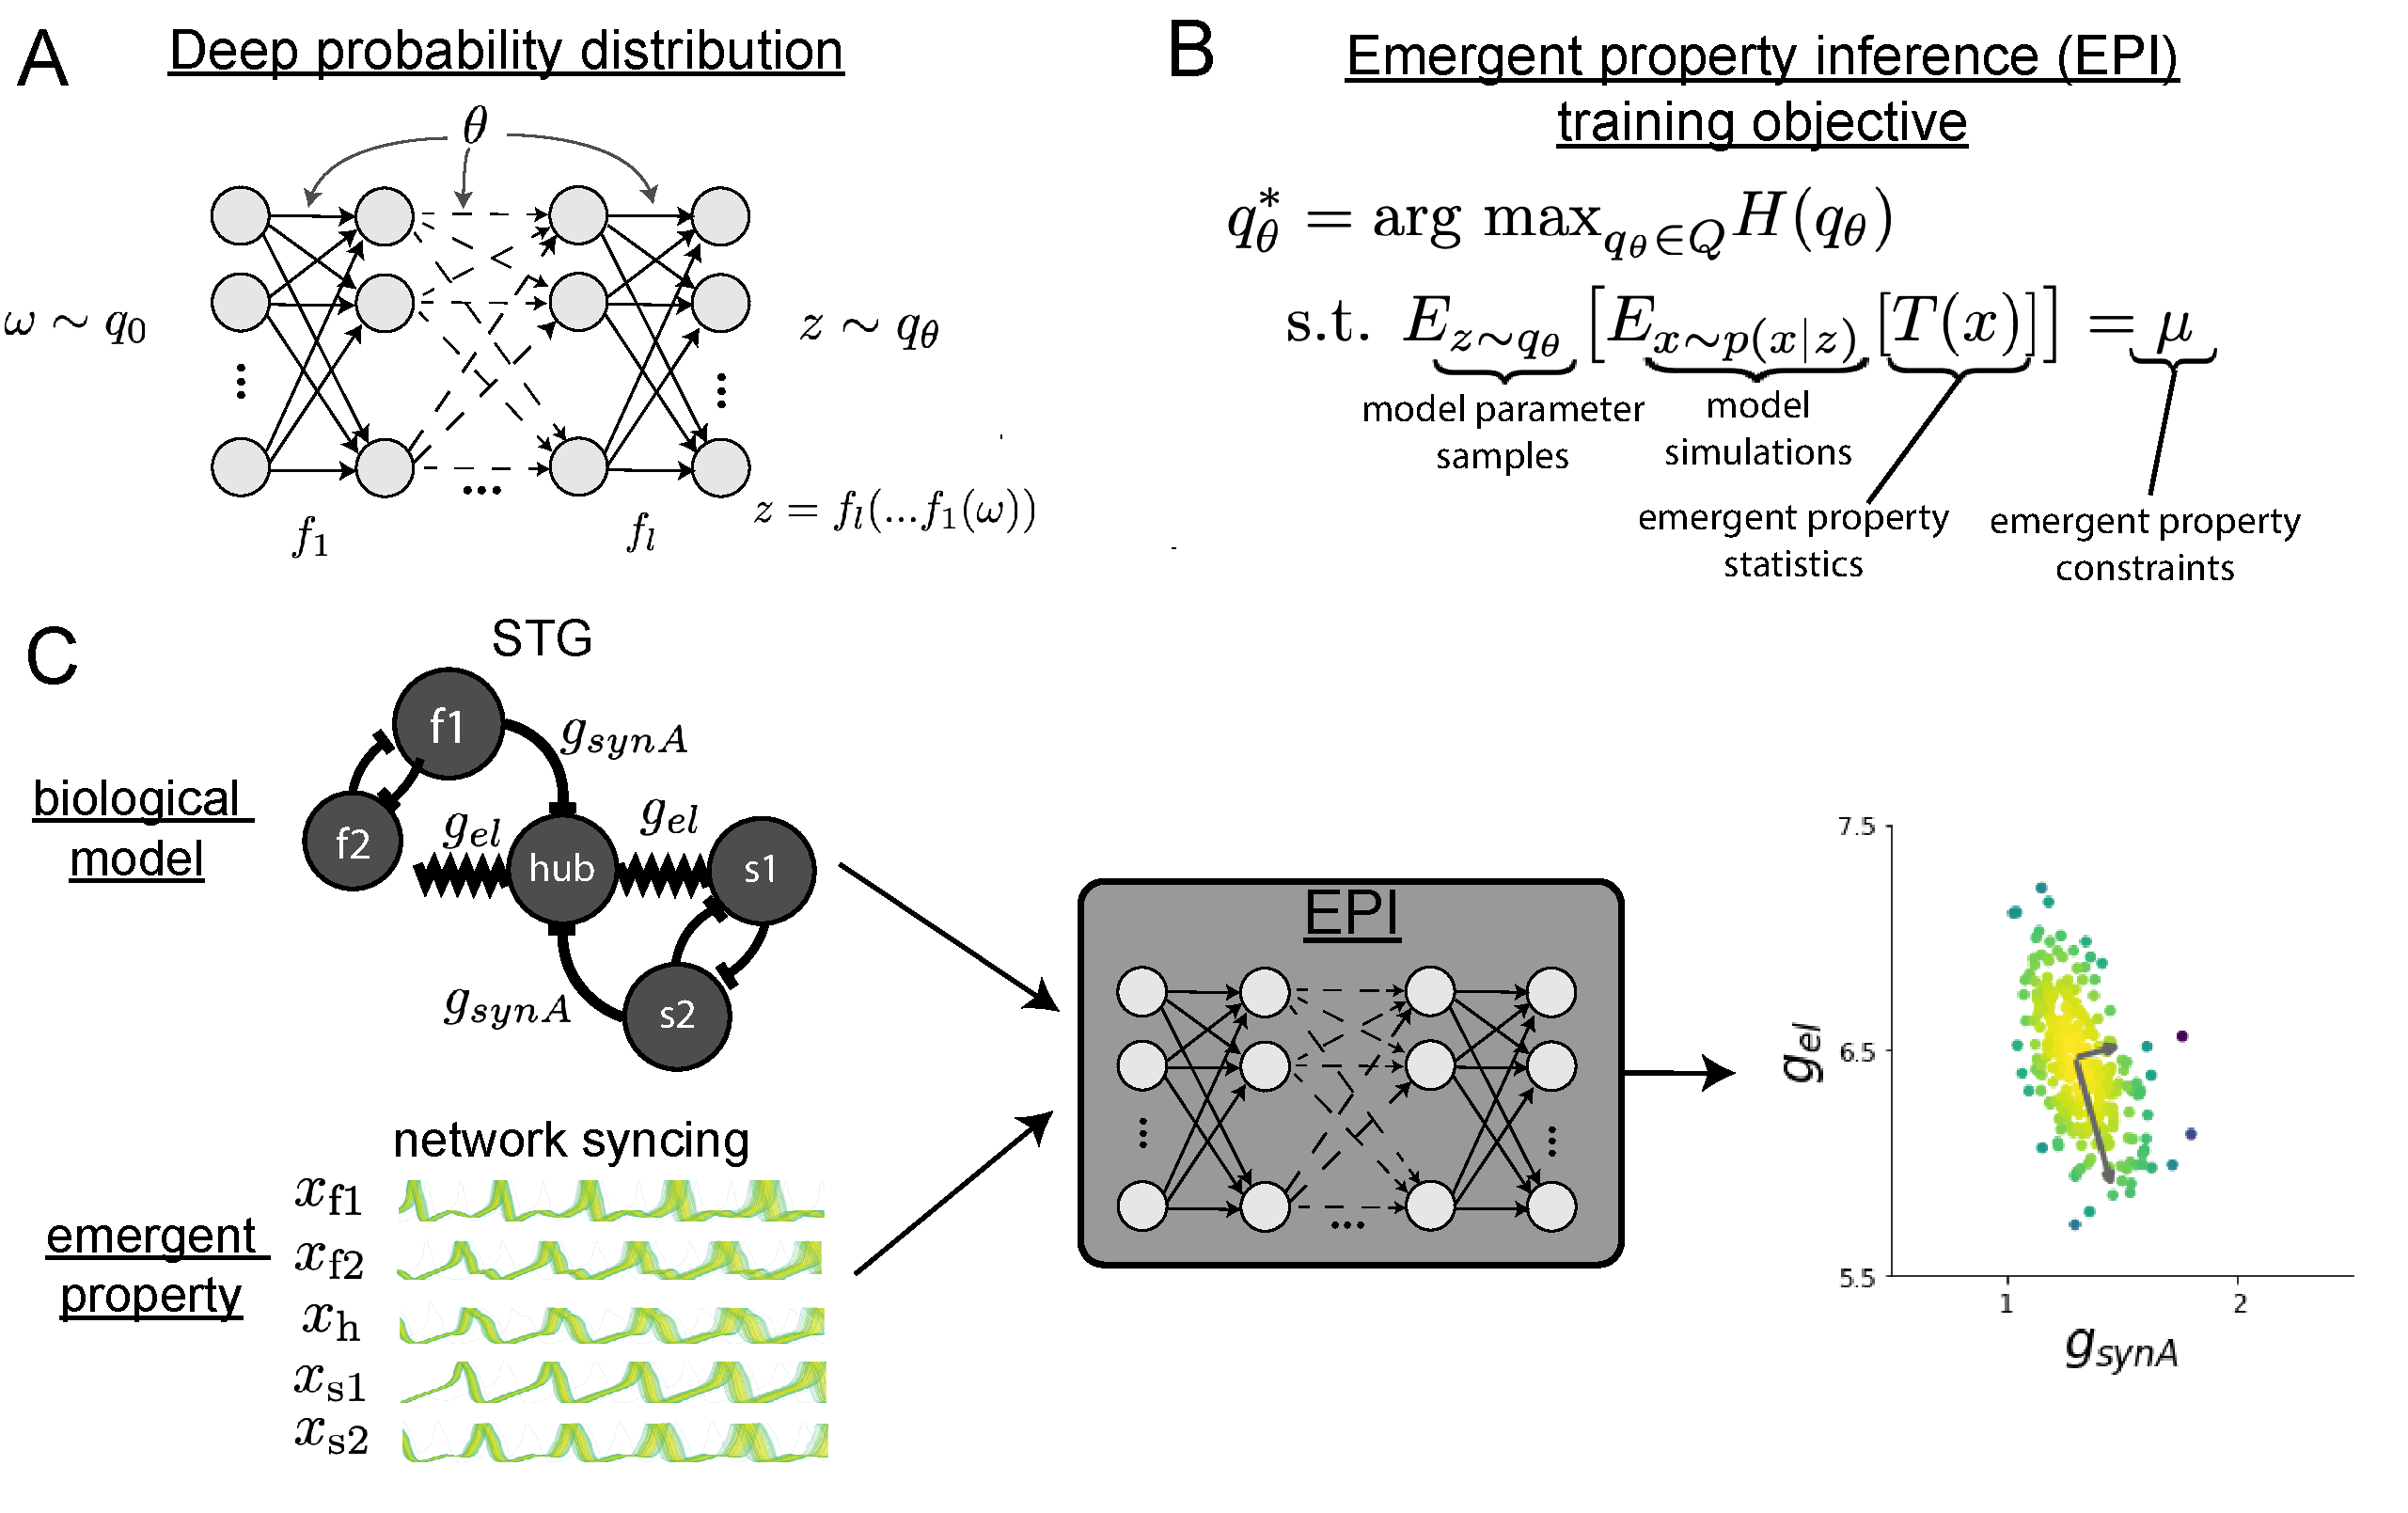
\includegraphics[scale=0.4]{figs/fig2/fig2.pdf}
\end{center}
\caption{A. Degenerate solution networks (DSNs) are deep probability distributions $q_\theta(z)$ of theoretical model parameterizations that produce emergent properties of interest.  The stochasticity of a deep probability distribution comes from a simple random variable $\omega \sim q_0$, where $q_0$ is often chosen to be an isotropic gaussian, and the structure comes from the deterministic transformation made by the deep neural network with optimized parameters $\theta$.  DSNs are the result of a constrained stochastic optimization, in which emergent properties $T(x)$ are fixed in expectation over model simulations $x \sim p(x \mid z)$ and DSN samples $z \sim q_\theta(z)$ to be a particular value $\mu$.  DSNs distributions maximize randomness through entropy. B. For a choice of model (STG) and emergent property (network syncing), a DSN learns a posterior distribution of the model parameters  $z = \left[g_{\text{el}}, g_{\text{synA}} \right]^\top$ conditioned on network syncing.}
\end{figure}

\subsection{Parametric robustness in the stomatogastric ganglion}
The stomatogastric ganglion (STG) of crustaceans is a small neural circuit, which generates multiple rhythmic muscle activation patterns for digestion \cite{marder}. The evolution of STG neuron membrane potentials are well-described by a theoretical model, where dynanical state $x = \begin{bmatrix} x_{\text{f1}}, x_{\text{f2}}, x_{\text{hub}}, x_{\text{s1}}, x_{\text{s2}} \end{bmatrix}^\top$ is the membrane potential for each neuron, which evolves by the biophysical conductance-based equation
\begin{equation} C_m \frac{\partial x}{\partial t} = - \left[ h_{leak} + h_{Ca} + h_K + h_{hyp} + h_{elec} + h_{syn}\right] 
\end{equation} 
where $C_m$=1nF, and $h_{\text{leak}}$, $h_{Ca}$, $h_K$, $h_{\text{hyp}}$, $h_{\text{elec}}$, $h_{\text{syn}}$ are the leak, calcium, potassium, hyperpolarization, electrical, and synaptic currents, respectively (see Methods).
Theoretical work has been done to characterize how model parameters such as the electical conductance $g_{\text{el}}$ and synaptic conductance $g_{\text{synA}}$ govern the production of these rhythms using visualization of statistics of simulated membrane potentials. \cite{gutierrez2013multiple}.  In this 5-neuron model,  two fast neurons ($f1$ and $f2$) mutually inhibit one another, and oscillate at a faster frequency than the slow neurons ($s1$ and $s2$), which also mutually inhibit each other  (Fig. 2C, top-left).   There is an interesting parameter regime of circuit activity, in which all neurons phase lock and oscillate at an intermediate synced frequency.

With EPI, we are able to learn a distribution of the STG conductance parameters $z = \left[g_{\text{el}}, g_{\text{synA}} \right]^\top$  that produce the emergent property of network syncing (Fig. 2C).  In order to execute EPI, we first select the 5-neuron STG as our theoretical model and network syncing emergent property of interest. To obtain a differentiable calculation of the firing frequencies (the emergent property statistics) given the model parameters (the conductances), we use soft-selection of a complex exponential basis applied to the simulated membrane potentials (see Methods).  This gradient is then used by the EPI algorithm to learn an approximate posterior distribution of the conductance parameters.

Once we have run EPI, we can immediately identify dimensions of parameter space that are sensitive (or degenerate) with respect to network syncing by evaluating the Hessian of the DSN distribution at the mode (Fig. 2C, right).  The arrows indicate the direction of eigenvectors of the Hessian, and their length is inversely proportional to the magnitude of the corresponding eigenvalue (long and short correspond to degenerate and sensitive, respectively).  Indeed, the Hessian eigenvector with greater eigenvalue is sensitive to network syncing (Fig. S1). 

\subsection{Comprehensive input-responsivity in a nonlinear sensory system}
Dynamical models with two populations (excitatory (E) and inhibitory (I) neurons) of visual processing have been used to reproduce a host of experimentally documented phenomena in primary visual cortex (V1).  In particular regimes of excitation and inhbition, these models exhibit the paradoxical effect \cite{tsodyks1997paradoxical}, selective amplification \cite{murphy2009balanced}, surround suppression \cite{ozeki2009inhibitory}, and  sensory integrative properties \cite{rubin2015stabilized}.  Since I neurons mostly fall into one of three classes (parvalbumin (P)-, somatostatin (S)-, and vasointestinal peptide (V)-expressing neurons) \cite{markram2004interneurons, rudy2011three}, theorists look to extend these dynamical models to four populations \cite{litwin2016inhibitory} (Fig. 3A).

The dynamical state of this model is the firing rate of each neuron type population $x = \begin{bmatrix} x_E & x_P & x_S & x_V \end{bmatrix}^\top$, which evolves according to rectified, exponentiated dynamics:
\begin{equation}
\tau \frac{dx}{dt} = -x + [W x+ h]_+^n
\end{equation}
with effective connectivity weights $W$, input $h$, time constant $\tau = 20ms$, and dynamics coefficient $n = 2$.  
We can obtain an informative estimate of the effective connectivities between these neuron types in mice by multiplying their probability of connection by the synaptic efficacy \cite{allen} (see Methods).
This brings us to a key question for this model: Given these fixed parameter choices of $W$, $n$, and $\tau$ and a baseline input $b$, what differential inputs to the system $dh = \begin{bmatrix} dh_E & dh_P & dh_S & dh_V \end{bmatrix}^\top$ drive each neuron type population where
\begin{equation}
h = b + dh
\end{equation}

Analytic approaches to studying nonlinear dynamical system are profoundly more complicated when moving from two-dimensional to three- or four-dimensional systems in the absence of restrictive simplifying assumptions \cite{strogatz1994nonlinear}. 
Yet, we are at least able to obtain via analysis the linearized response to input of the system $\frac{dx_{ss}}{dh}$ at a given fixed point (see Methods).  
While this linear prediction is accurate for small differential inputs (Fig. 3B, left), it is often misleading in such nonlinear models as differential input strength increases (Fig. 3B, right). In fact, for a baseline input of $b = \begin{bmatrix} 1 & 1 & 1 & 1 \end{bmatrix}^\top$ the linearly predicted response for $dh = \begin{bmatrix} 0.5 & 0.5 & 0.5 & 0.5 \end{bmatrix}^\top$ is actually in the opposite direction for the V-population (Fig. 3B, right, green).

To get a more comprehensive picture of the input-reponsivity of each neuron type, we use EPI to learn a distribution of inputs $dh$ that cause the rate of each neuron-type population $\alpha$ to increase by a value $y$ with some allowed variance.  We denote this emergent property of neuron-type responsivity as $\mathcal{B}(\alpha, y)$ (see Methods).  In Fig. 3C, each column visualizes the approximate posterior $dh$ corresponding to a specific neuron-type increase, while each row corresponds to amounts of increase 0.1 and 0.5.  Akin to the practice of exploratory analysis of neural data sets, in which we search for meaningful structure, we can do an exploratory analysis of this \emph{model} yielding a meaningful understanding of its operation.

To visualize these four-dimensional distributions, we pairplot the two-dimensional marginal densities, which yield an insightful picture.  Primarily, there are salient sensitivities and degneracies in $dh$ with respect to neuron-type firing rate increases.  Of course, each neuron-type is sensitive to its direct input.  The E- and P-population are largely unaffected by $dh_V$, and the S-population is also largely unaffected by $dh_P$ for the rate increases examined.  Secondly, we observe a stabilization role by the P-population with respect to the E- and V-populations (the two it projects to besides itself).  This deduction is supported by the tight positive correlation between $dh_P$ and $dh_E$ for E-population increases and also between $dh_P$ and $dh_V$ for V-population increases.

One may naively expect that increasing input to the E-population will increase the activity of the inhibitory populations, but this is far from the case. In actuality, EPI shows that negative $dh_E$ results in small inhibitory firing rate increases.  However, for a larger increase from the V-population, a positive $dh_E$ is required.

All of this insight was gained beyond what the analytic linear prediction told us (cyan lines that you can't see).  
By flexibly conditioning on different emergent properties (the responses of each neuron type population), we were able to gain an informative understanding of this model.
In the next section, we show how systematically conditioning on different values of an emergent property statistic can yield powerful conclusions about theoretical models and produce experimentally testable predictions.

\begin{figure}
\begin{center}
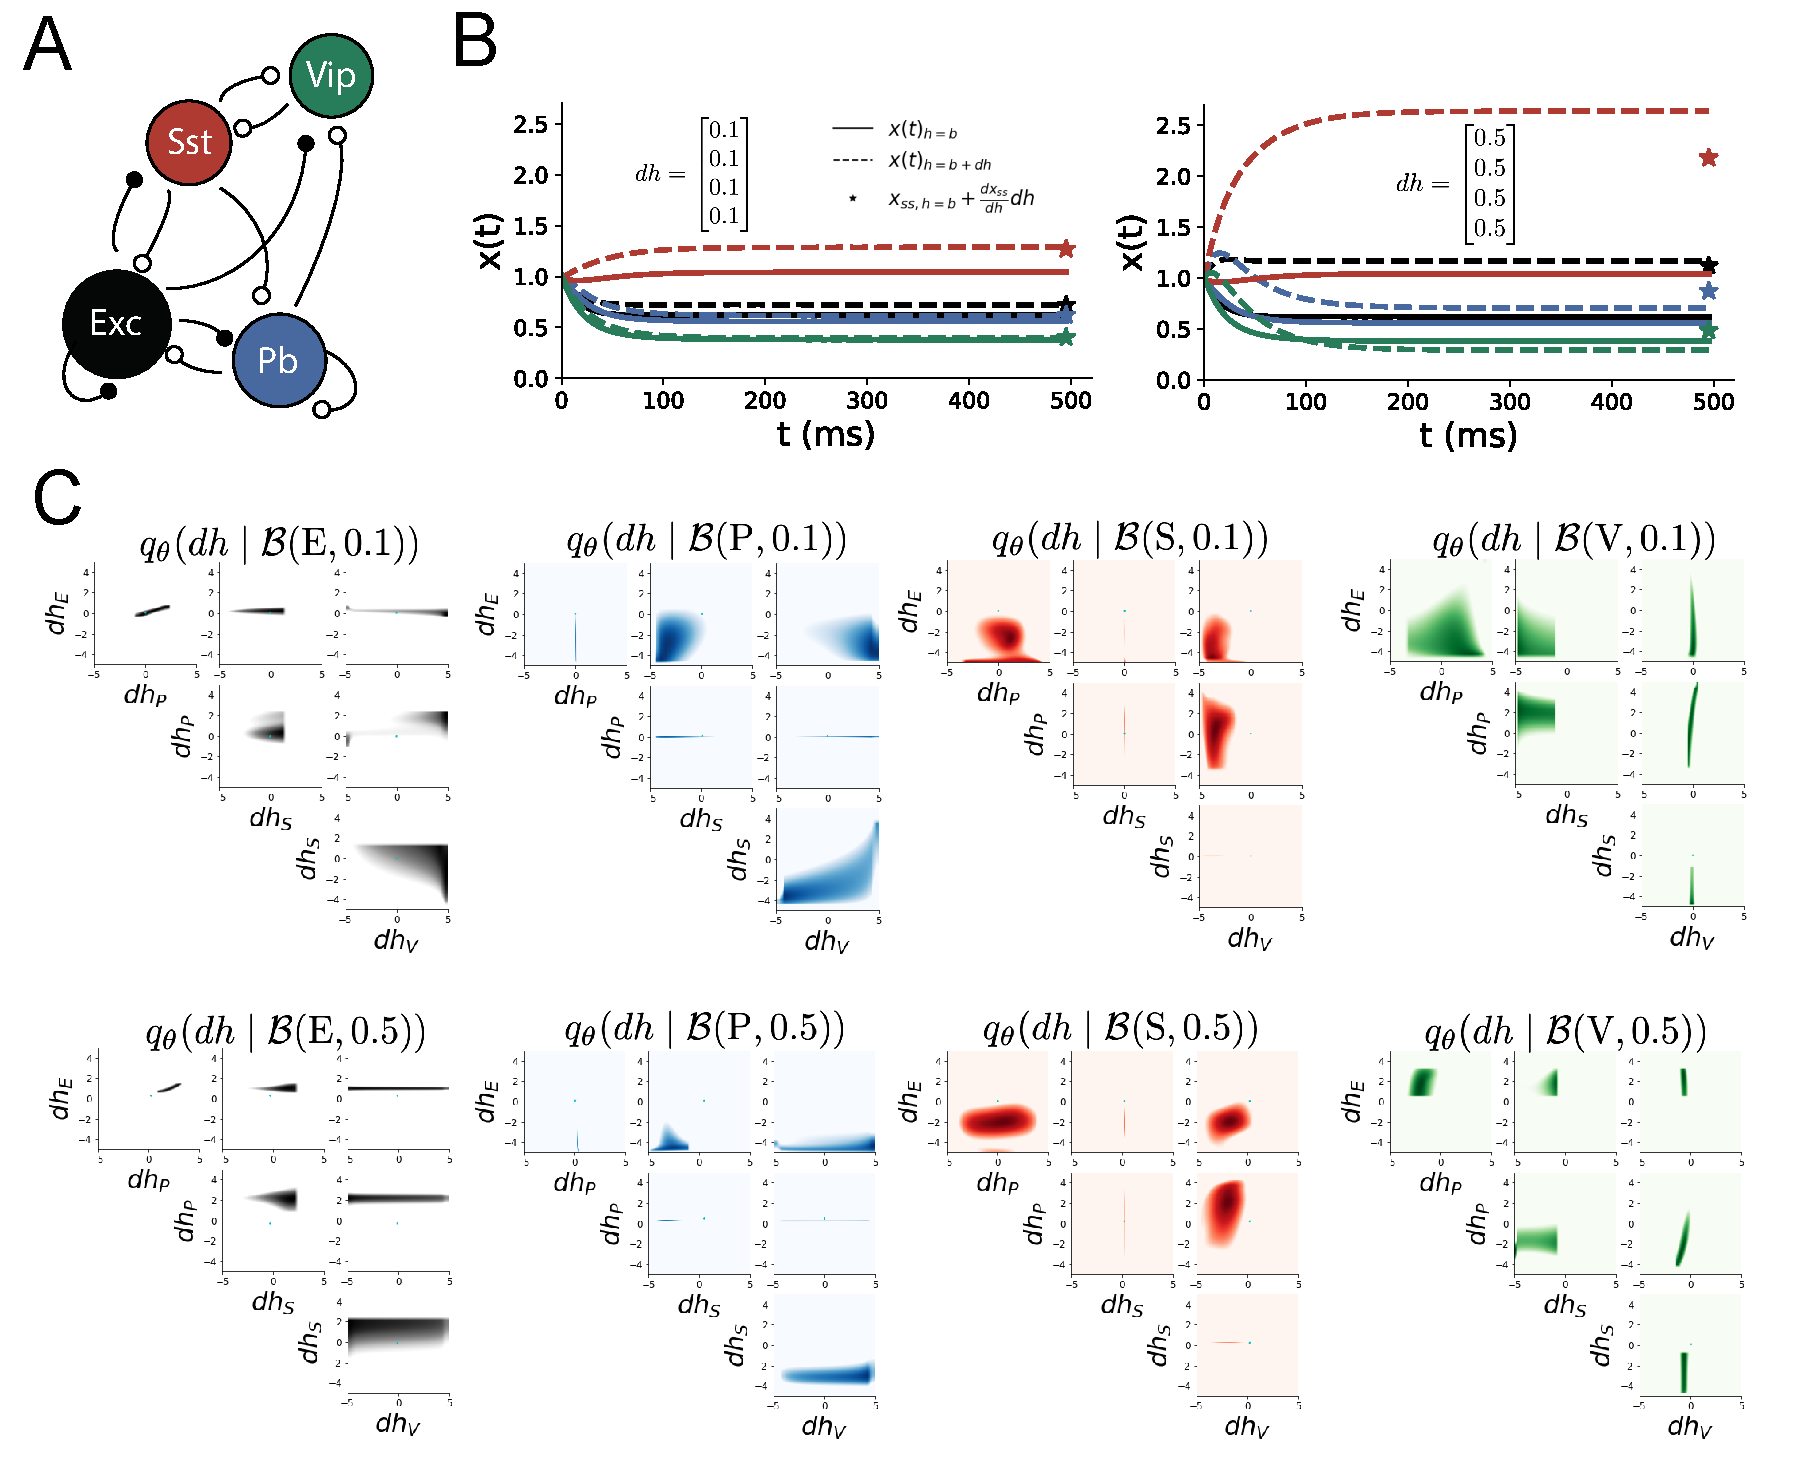
\includegraphics[scale=0.5]{figs/fig3/fig3.pdf}
\end{center}
\caption{A. V1 model B. Responses and why linear isnt good enough. C. DSN stuff.}
\end{figure}

\subsection{Identifying neural mechanisms of behavioral learning.} 
A key challenge for theorists modeling neural circuits underlying cognitive behavior is the description of sufficient changes to biologically meaningful parameters that result in improved behavoir.
Identifying measurable biological changes that should occur for increased performance is critical for neuroscience, since they may indicate how the learning brain adapts.  
In a rapid task switching experiment, where rats are to respond right (R) or left (L) to the side of a light stimulus in the pro (P) task, and oppositely in the anti (A) task predicated by an auditory cue (Fig. 4A), neural recordings exhibited two population of neurons in each hemisphere of superior colliculus (SC) that simultaneously represented both task condition and motor response: the pro/contra and anti/ipsi neurons \cite{duan2018collicular}.  Duan et al. propose a four-population dynamical model of superior colliculus with a Pro- and Anti-population in each hemisphere, where activities are bounded from 0-1, and a high output of the Pro population in a given hemisphere corresponds to the  contralateral response. The connectivity matrix is parameterized by the geometry of the population arrangement (Fig. 4B). Here, we use EPI to learn connectivities consistent with varying degrees of rapid task switching accuracy, resulting in experimentally testable predictions on how connectivity in SC changes while learning this behavioral paradigm.

\begin{figure}
\begin{center}
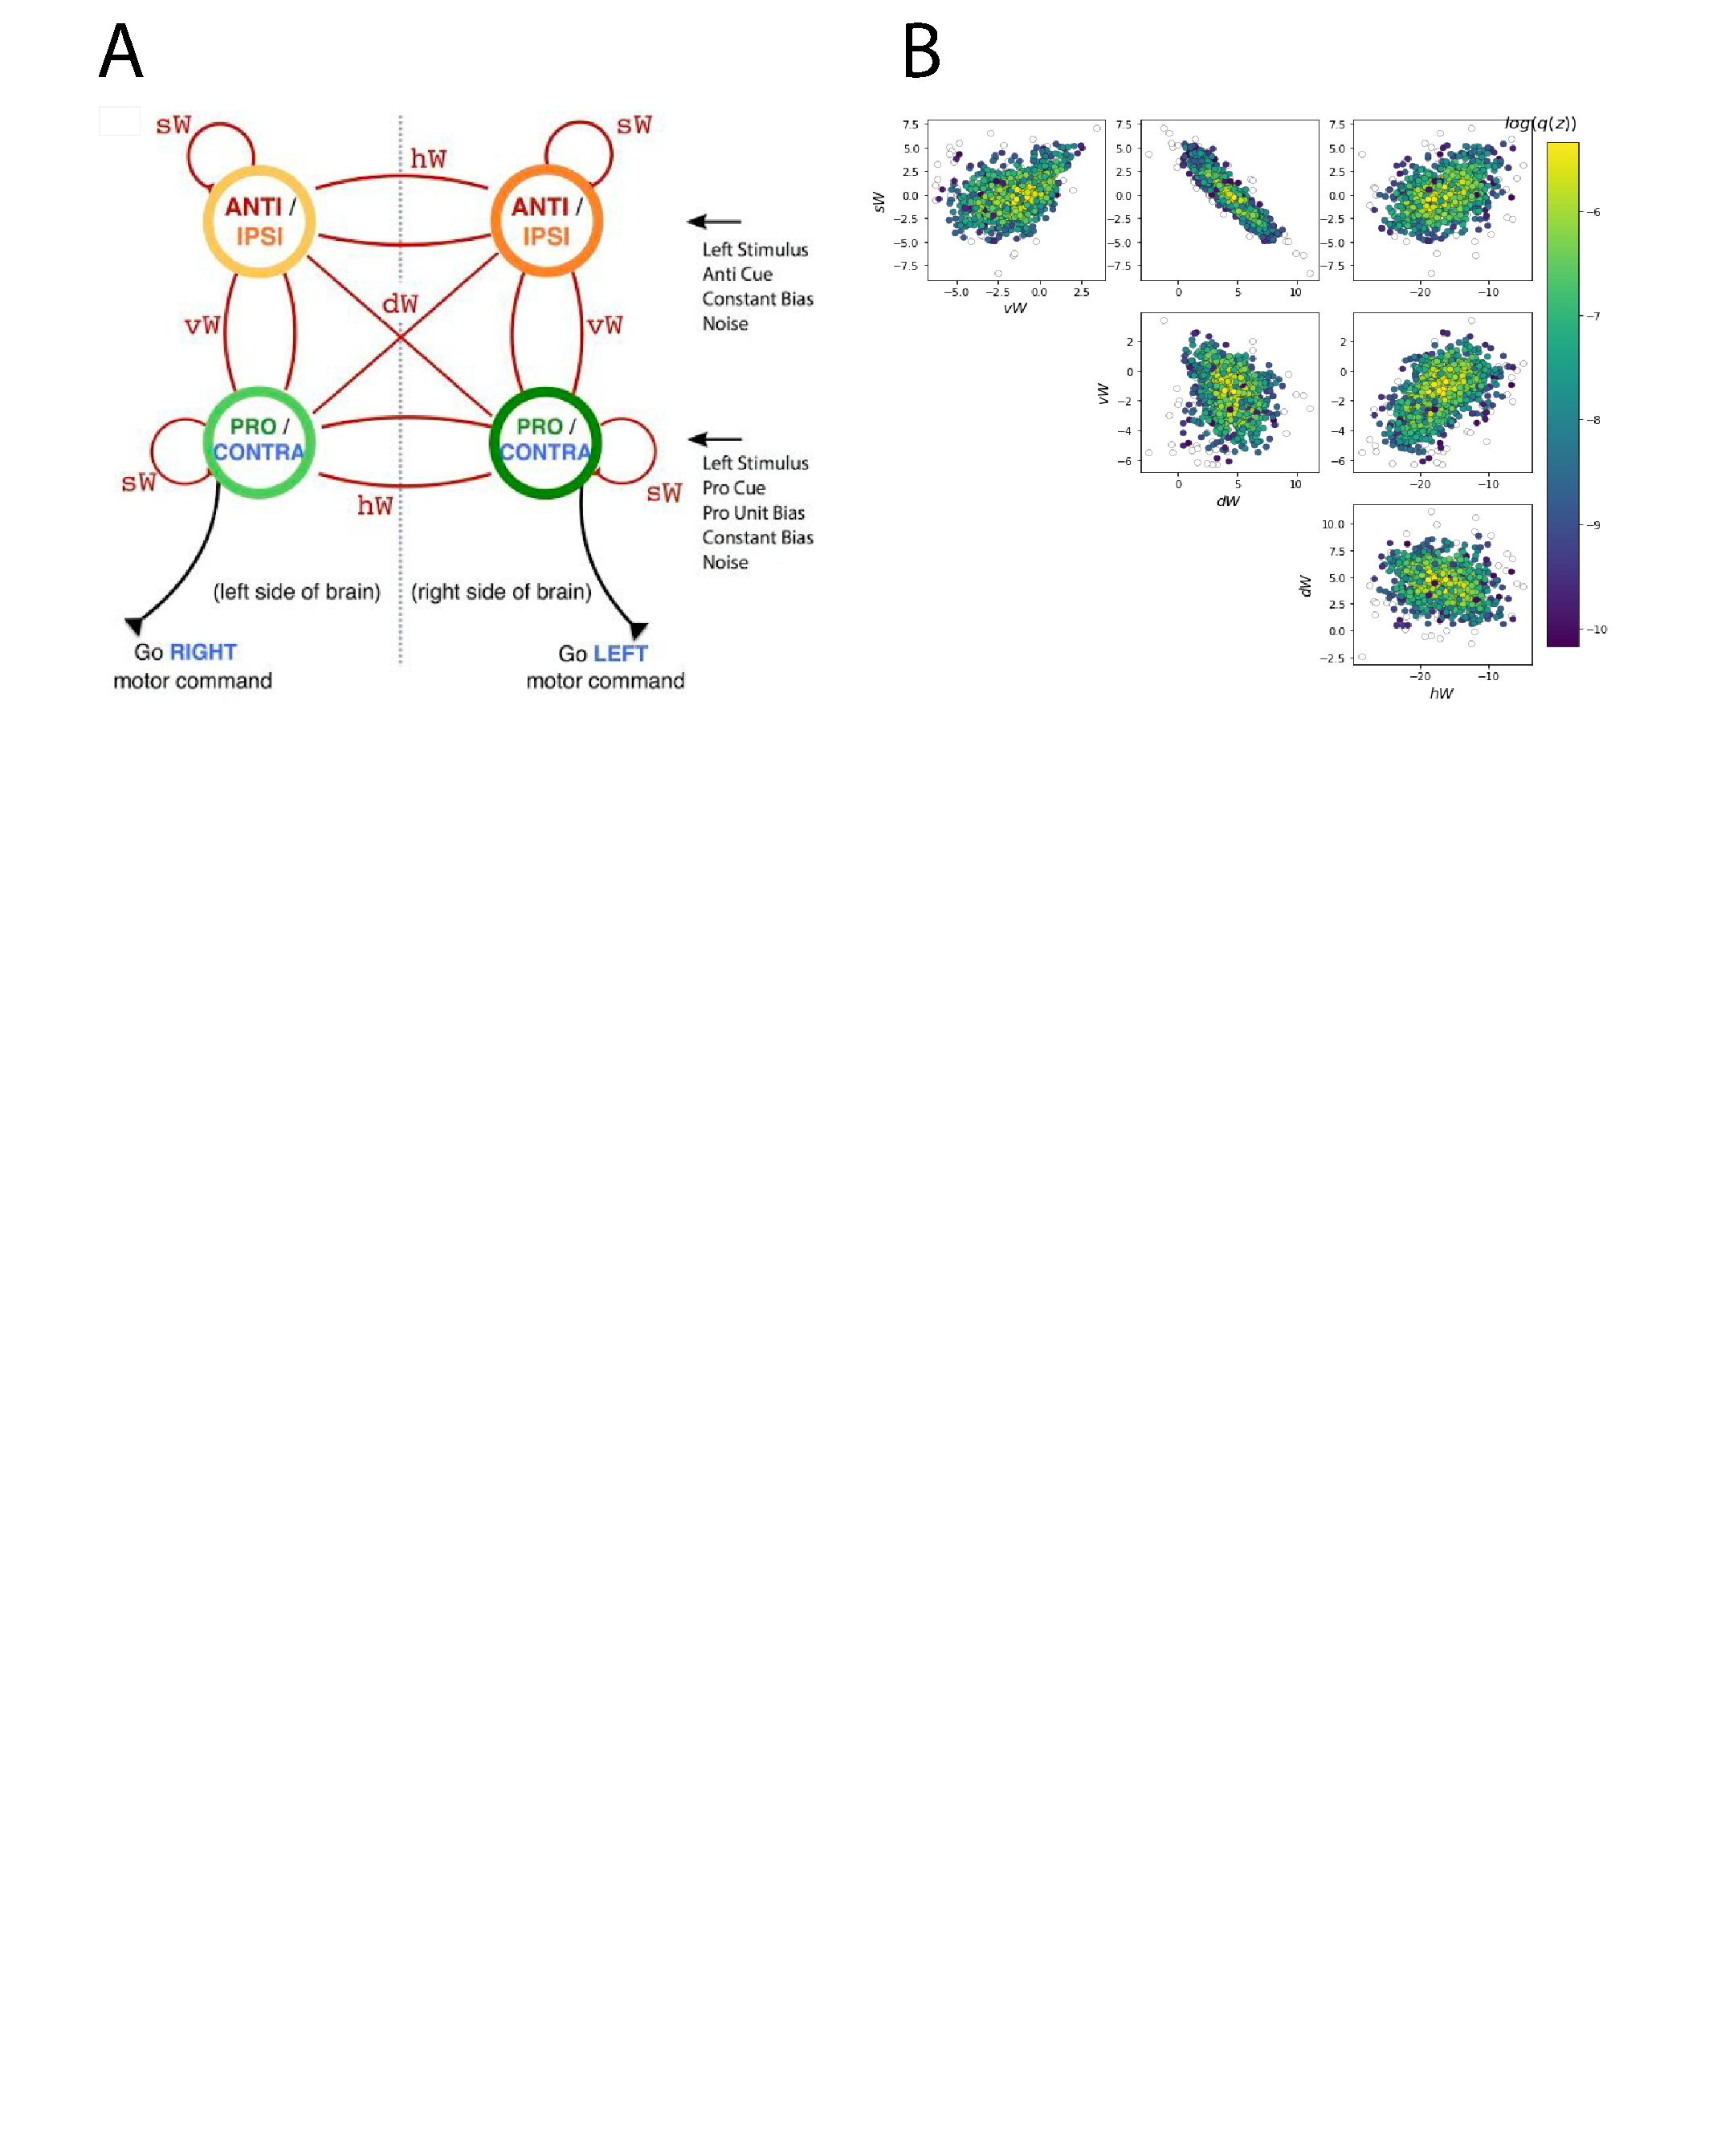
\includegraphics[scale=0.4]{figs/fig4/fig4.pdf}
\end{center}
\caption{A. Rapid task switching behavioral paradigm. In the Pro (Anti) condition indicated by an auditory cue, the rats are to respond to the same (opposite) side as the light stimulus that is provided after a delay to receive a reward. B. Model of superior collicullus (SC). Neurons: LP - left pro, RP - right pro, LA - left anti, RA - right anti.  Parameters: sW - self, hW - horizontal, vW -vertical, dW - diagonal weights. C. The Schur decompostion of the weight matrix. D. The marginal EPI posteriors of the Schur eigenvalues at each level of task accuracy.}
\end{figure}

We ran EPI to learn appproximate posteriors of SC model weight matrix parameters $z = W$ conditioned on of various levels of rapid task switching accuracy $\mathcal{B}(p)$ for $p \in \{50\%, 60\%, 70\%, 80\%, 90\%\}$ (see Methods).  The Schur decomposition of the weight matrix, a unique decomposition revealing the underlying directed structure between modes (the eigenvectors), has the same eigenvectors for all $W$s under this symmetric parameterization (Fig. 4C).
These consistent Schur eigenvectors have intuitive roles in processing for this task, and the corresponding eigenvalues $a$ of each mode (which change according to $W$ indicate the amplification or supression of activity along that mode.  These Schur eigenvectors have intuitive roles with respect to processing in this task, and are accordingly named the \textit{all}, \textit{side}, \textit{task}, and \textit{diag} modes. 

As learning progresses, the task mode is increasingly amplified, indicating the criticality of a distributed task representation at the time of stimulus presentation, (Fig. 4D, purple).  Stepping from task-naive 50\% networks to task-performing 60\% networks, there is a marked suppression of the side mode (Fig. 4D, orange).  Such side mode suppression remains in the regimes of greater accuracy, revealing its importance towards the existence of a distributed task representation.   Across all learning regimes, the diag mode is amplified (Fig. 4D, cyan), and the all mode is suppressed (Fig. 4D, black), which can be seen as signatures of Bernoulli winner-take-all networks (see Methods).  We can conclude that side mode suppression allows rapid task switching, and that greater task-mode representation increases accuracy (Fig. S3).  These findings motivate experimental predictions, in which we would expect the effective connectvity between these populations to change throughout learning in a way that increases the task mode and decreses the side mode eigenvalues.

\subsection{Characterizing the sources of bias during approximate inference in RNNs}
At a more abstract level, recurrent neural networks (RNNs) are high-dimensional models of computation, which have become increasingly popular in systems neuroscience research \cite{barak2017recurrent}. 
Typically, RNNs are trained to do a task from a systems neuroscience experiment, and then the latent factors of the trained RNN are compared to recorded neural activity.  
Recent theoretical work proceeding in that direction extends dynamic mean field theory (DMFT) from random \cite{sompolinsky1988chaos} to low rank RNNs \cite{mastroguiseppe2018linking}.
This theory establishes a link between interpretable, geometric parameterizations of the RNN connectivity with the emerging dynamics.

\begin{figure}
\begin{center}
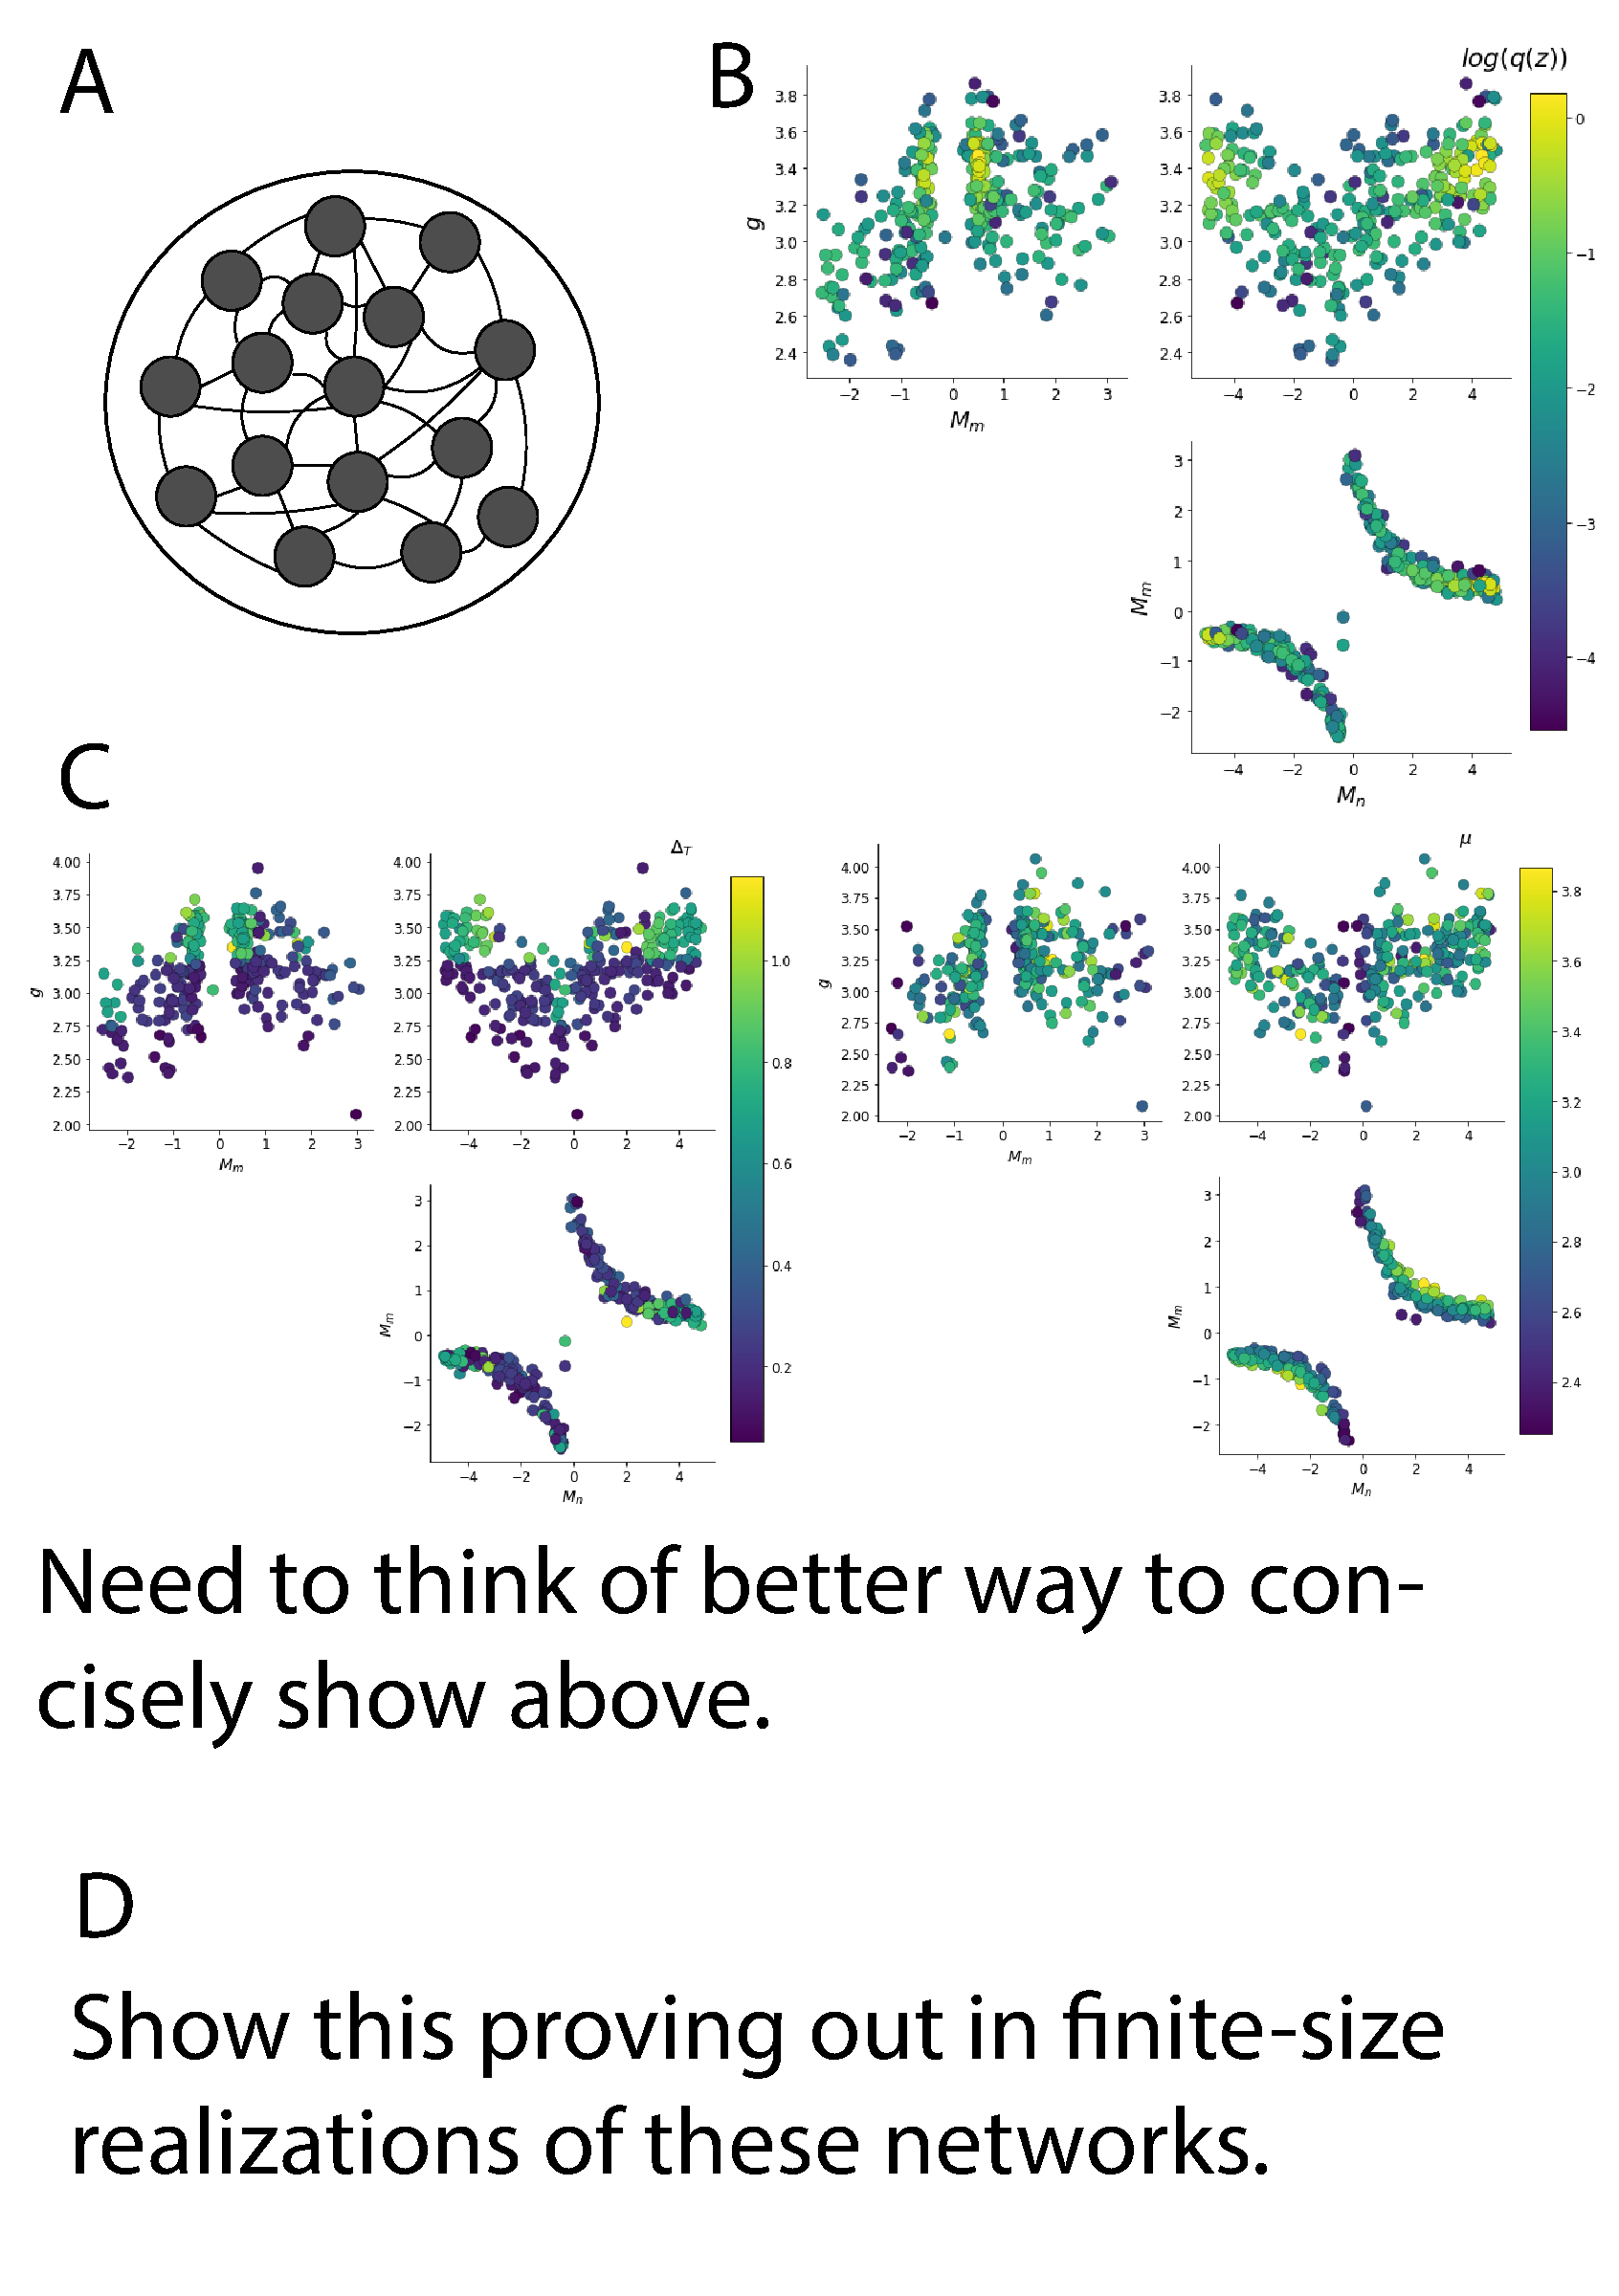
\includegraphics[scale=0.6]{figs/fig5/fig5.pdf}
\end{center}
\caption{A. RNN. B. LRRNN DSN.  C. Visualizing how the params affect the bias.  D. Finite size realizations proving out the DMFT theory.}
\end{figure}

Here, we use this theory along with EPI to characterize the mechanistic sources of bias during approximate Bayesian inference in a rank-1 RNN. The rank-1 RNN's connectivity is the sum of a random component with strength determined by $g$, and a structured component determined by vectors $m$ and $n$:
\begin{equation}
J = g\chi + \frac{1}{N}mn^\top
\end{equation}
where $\chi_{ij} \sim \mathcal{N}(0, \frac{1}{N})$ and $m_i \sim \mathcal{N}(M_m, 1)$ and $n_i \sim \mathcal{N}(M_n, 1)$.  The Bayesian inference problem for the rank-1 RNN to solve is to estimate a posterior on the mean of some gaussian distributed observations $x \sim \mathcal{N}(\mu_x, \sigma_x^2)$ given a prior of $\mu_x \sim \mathcal{N}(4, 1)$ (Fig. 5A).  When the observations take the distribution $x \sim \mathcal{N}(2, 1)$, the true posterior is $\mu_x \sim \mathcal{N}(\mu_{\text{post}}=3, \sigma^2_{\text{post}}=0.5)$.  To execute approximate inference, we require that the rank-1 RNN produce its estimate of gaussian posterior mean and variance with its mean activity $\mu$ and amount of temporal variance $\Delta_T$, respectively (see Methods).

We use EPI to learn the distribution of $z = \begin{bmatrix} g & M_m & M_n \end{bmatrix}^\top$ that produces a distribution of rank-1 RNNs executing approximate Bayesian inference. 
Intentionally, we include a substantial amount of variability in the second moment constraints of the network mean $\mu$ and temporal variance $\Delta_T$ to get an variety of types of bias in the sampled rank-1 RNNs.  
The posterior distribution is roughly symmetric in the $M_m$-$M_n$ plane which structure suggesting there is a degeneracy with respect to approximate Bayesian inference in the product of $M_m$ and $M_n$ (Fig. 5B).  
The product of $M_m$ and $M_n$ almost completely determines the posterior mean (Fig. 5B, left), and the random strength $g$ is the most influential variable on the temporal variance (Fig. 5B, right). 
 Neither of these observations are obvious from the consistency equations afforded by DMFT (see Methods), the solvers of which we took gradients through to run EPI.  
 
Finite-size realizations of networks from this posterior distribution indeed have the biases in their approximate inference procedures indicated by the DMFT (Fig. 5C). The network with parameter $z_1$ produces an overestimate of th  posterior mean and variance, while the network with parameter $z_2$ produces underestimates.  This novel procedure of doing inference in interpretable parameterizations of RNNs conditioned on abstract cognitive tasks can be generally executed on other tasks like noisy integration and context-dependent decision making (Fig. S4).

\subsection{EPI is a general tool for all of theoretical neuroscience}
For decades, we have used statistical machine learning to discover meaningful structure in neural data sets.  Theoretical neuroscience has not appreciably been affected by these tools for technical reasons, but now that doesn't need to be the case.  When working in settings of close biological realism, with complex nonlinear dynamics, we show that we are still able to use modern deep learning techniques to produce a novel characterization of parameteric robustness in a model of the STG. Of course, this approach is not specific to models of serious biological realism, as we've shown application to RNNs, which are quite abstract.  We are able to condition both deterministic and stochastic models on all sorts of  emergent properties from membrane potential firing to execution of approximate inference, so long as these emergent property statistics are continuously differentiable with respect to the model parameters.

There are important technical considerations when considering the suitability of EPI for a particular modeling question.  First, how computationally expensive is the gradient of the emergent propety statistic with respect to the model parameters.  In the most suitable of cases, there is a simple closed form expression (ref linear 2d appendix section).  On the other end of the spectrum, you may require many a large number simulation iterations before a high quality measurement of the emergent property statistic is available as in measuring firing frequency in the STG (ref Methods section for STG).  In such cases, optimization will be expensive, and it is worth considering an alternative methodology (ref to appendix on this topic).   Secondly, the defined emergent property should not be under- or overconstrained.  If underconstrained, the posterior will will grow (in entropy) unstabily unless mapped to a finite support.  If overconstrained, and there is no support producing the emergent property, learning will fail.

\section{Discussion}

 Talk big picture: If we know we can't analytically derive these things, we need an alternative characterization.  Simulate and examine isn't cutting it.  We need to be leveraging the modern inference engine to gain this understanding.  

In consideration of experimental measurements of the effective connectivity (via probability of connection and estimation of synaptic efficacy) between pro/contra and anti-ipsi neurons in rat SC at various stages of task peformance throughout learning, we would predict an initial reduction in side mode eigenvalue, and a steady increase in task mode eigenvalue of such effective connectivity matrices.   While experimentally testable predictions are highly valuable, sometimes it is prohibitively challenging to design a biologically realistic model of a neural computation. In the next section, we show how to perform statistical inference on interpretable parameterizations of more general, abstract models of neural computation.

The scientific philosophy is as follows: optimize an RNN to execute a task from behavioral neuroscience, compare the activity of this optimized system to brain activity of a model organism doing the same task, and leverage the full observability of the trained RNN to generate hypotheses of the neural mechanisms of computation.  While fixed point identification and jacobian measurement yield intuitive portraits of the implemented computational algorithm, there is dizzying degeneracy in the RNN connectivity matrix with respect to these characterizations.  To develop an understanding of the neural mechanisms at play, we must work in a reduced, interpretable parameter setting of these powerfully general models \cite{doya1993universality}.

Para about what we can achieve with LRRNNs and EPI.

Expand on idea of posterior predictive checks / hypothesis testing / exploratory analyses of models themselves.  Give the whole, we don't even understand the models we're developing pitch.

%\item Link conditioning on task execution with work done today with RNNs.  Although there seems to be consistency across RNN archs \cite{universality2019Maheswaranathan}, basically we're training overparameterized models with regression, and get a distribution (we have no prob treatment of). Emphasize utility of low-dim interpretable parameterizations. RNNs are particularly useful, when an interpretable model can not easily be designed to execute a task/behavior of interest. Other relevant work \cite{zhao2016interpretable, duncker2019learning}.
%Elaborate on idea of conditioning on flexibly defined statistics i.e. emergent properties. Emphasize how this is practical.  Link to sufficient statistics, esp. commonly used in phenom models like spike counts etc.
%A paragraph on bridging large scale recordings with theory.


\bibliography{NN2019}
\bibliographystyle{unsrt}

\appendix

\section{Supplement}

\subsection{Degenerate solution networks (DSNs)}
DSNs learn distributions of theoretical model parameters that produce emergent properties of interest.  They combine ideas from likelihood-free variational inference (cite Dustin) and maximum entropy flow networks (cite Gabe).  A maximum entropy flow network is used as a deep probability distribution for the parameters, while these samples are passed through a differentiable model/dynamics simulator, which can lack a tractable likelihood function.

Consider model parameterization $z$ and data $x$ generated from some theoretical model simulator represented as $p(x \mid z)$, which may be deterministic or stochastic.  Neural circuit models usually have known sampling procedures for simulating activity given a circuit parameterization, yet often lack an explicit likelihood function for the neural activity due to having nonlinear dynamics. DSNs learn a distribution on parameters $z$, that yields a behavior of interest $\mathcal{B}$,
\begin{equation}
\mathcal{B}: E_{z \sim q_\theta}\left[ E_{x\sim p(x \mid z)}\left[T(x)\right] \right] = \mu
\end{equation}
by making an approximation $q_\theta(z)$ to $p(z \mid \mathcal{B})$ (see Section A.1.5).  So, over the DSN distribution $q_\theta(z)$ of model $p(x \mid z)$ for behavior $\mathcal{B}$, the emergent properties $T(x)$ are constrained in expectation to $\mu$.

 In deep probability distributions, a simple random variable $w \sim p_0$ is mapped deterministically via a function $f_\theta$ parameterized by a neural network to the support of the distribution of interest where $z = f_{\theta}(\omega) = f_l(..f_1(\omega))$.  Given a theoretical model $p(x \mid z)$ and some behavior of interest $\mathcal{B}$, DSNs are trained by optimizing the neural network parameters $\theta$ to find the optimal approximation $q_{\theta}^*$ within the deep variational family $Q$ to $p(z \mid \mathcal{B})$.

In most settings (especially those relevant to theoretical neuroscience) the likelihood of the behavior with respect to the model parameters $p(T(x) \mid z)$ is unknown or intractable, requiring an alternative to stochastic gradient variational bayes (cite Kingma Welling 2013) or black box variational inference (cite Ranganeth 2014).  These types of methods called likelihood-free variational inference (LFVI, cite Tran) skate around the intractable likelihood function in situations where there is a differentiable simulator. Akin to LFVI, DSNs are optimized with the following objective for a given generative model and statistical constraints on its produced activity:

\begin{equation}
\begin{split}
q_\theta^*(z) &= \argmax_{q_\theta \in Q} H(q_\theta(z)) \\
 &  \text{s.t.  } E_{z \sim q_\theta}\left[ E_{x\sim p(x \mid z)}\left[T(x)\right] \right] = \mu \\
 \end{split}
\end{equation}

\subsubsection{Example: 2D LDS}
To gain intuition for DSNs, consider two-dimensional linear dynamical systems, $\tau \dot{x} = Ax$ with 
\[A = \begin{bmatrix} a_1 & a_2 \\ a_3 & a_4 \end{bmatrix}\]
 that produce a band of oscillations. To train a DSN to learn the maximally entropic distribution of real entries of the dynamics matrix $z = \left[a_1, a_2, a_3, a_4 \right]$, ($\tau=1$,) that yield a band of oscillations, $T(x)$ is chosen to contain the first- and second-moments of the oscillatory frequency $\Omega$ and the the primary growth/decay factor $d$ of the oscillating system.  To learn the distribution of real entries of $A$ that yield a $d$ around zero with variance 1.0, and oscillations at 1 Hz with variance 1.0, the behavior of DSN would be constrained to:
\begin{equation}
 \mu = E \begin{bmatrix} d \\ \Omega \\ d^2 \\ \Omega^2 \end{bmatrix} = \begin{bmatrix} 0.0 \\ 1.0 \\ 1.0 \\ 1.025 \end{bmatrix}
 \end{equation} 
We could simuilate system activity $x$ from $z$ for some finite number of time steps, and estimate $\Omega$ by e.g. taking the peak of the Discrete Fourier series.  Instead, the sufficient statistics for this oscillating behavior are computed through a closed form function $g(z)$ by taking the eigendecomposition of the dynamics matrix
\begin{equation}
g(z) = E_{x\sim p(x \mid z)}\left[T(x)\right] =  \begin{bmatrix} \text{real}(\lambda_1) \\ \frac{\text{imag}(\lambda_1)}{2 \pi} \\ \text{real}(\lambda_1)^2 \\ (\frac{\text{imag}(\lambda_1)}{2 \pi})^2 \end{bmatrix}
\end{equation}
\begin{equation}
\lambda = \frac{(\frac{a_1 + a_4}{\tau}) \pm \sqrt{(\frac{a_1+a_4}{\tau})^2 + 4(\frac{a_2 a_3 - a_1 a_4}{\tau})}}{2}
\end{equation}
where $\lambda_1$ is the eigenvalue of $\frac{1}{\tau}A$ with greatest real part.
Even though $E_{x\sim p(x \mid z)}\left[T(x)\right]$ is calculable directly via $g(z)$, we cannot derive the distribution $q^*_\theta$, since the backward mapping fromt the mean parameters $\mu$ to the natural parameters $\eta$ of his exponential family is unknown.  Instead, we can train a DSN to learn the degenerate linear system parameterization (Fig. S2B). Even this relatively simple system has nontrivial (though intuitively sensible) structure in the parameter distribution.\\

\subsubsection{Augmented Lagrangian optimization}
To optimize $q_\theta(z)$ in equation 1, the constrained optimization is performed using the augmented Lagrangian method.  The following objective is minimized:
\begin{equation}
L(\theta; \alpha, c) = -H(q_\theta) + \alpha^\top \delta(\theta) + \frac{c}{2}||\delta(\theta)||^2
\end{equation}
where $\delta(\theta) = E_{z \sim q_\theta}\left[ E_{x\sim p(x \mid z)}\left[T(x) - \mu \right] \right]$, $\lambda \in \mathcal{R}^m$ are the Lagrange multipliers and $c$ is the penalty coefficient.  For a fixed $(\alpha, c)$, $\theta$ is optimized with stochastic gradient descent.  A low value of $c$ is used initially, and increased during each augmented Lagrangian epoch. Similarly, $\alpha$ is tuned each epoch based on the constraint violations.  For the linear 2-dimensional system (Fig. S2C) optimization hyperparameters are initialized to $c_1 = 10^{-4}$ and $\alpha_1 = 0$.  The penalty coefficient is updated based on a hypothesis test regarding the reduction in constraint violation.  The p-value of $E[||\delta(\theta_{k+1})||] > \gamma E[||\delta(\theta_{k})||]$ is computed, and $c_{k+1}$ is updated  to $\beta c_k$ with probability $1-p$.  Throughout the project, $\beta = 4.0$ and $\gamma = 0.25$ is used.  The other update rule is $\alpha_{k+1} = \alpha_k + c_k \frac{1}{n} \sum_{i=1}^n (T(x^{(i)}) - \mu)$.  Each augmented Lagrangian epoch runs for 5,000 iterations.  We consider the optimization to have converged when a null hypothesis test of constraint violations being zero is accepted for all constraints at a significance threshold 0.05.  This is the dotted line on the plots below depicting the optimization cutoff of the DSN optimization for the 2-dimensional linear system.  If the optimization is left to continue running, entropy may decrease, and structural pathologies in the distribution may be introduced.

The intention is that $c$ and $\lambda$ start at values encouraging entropic growth early in optimization.  Then, as they increase in magnitude with each training epoch, the constraint satisfaction terms are increasingly weighted, resulting in a decrease in entropy.  Rather than using a naive initialization, before the DSN training, we otpimize the density network parameters to generate samples of an isotropic gaussian of a selected variance, such as 1.0 for the 2D LDS example.  This provides a convenient starting point, whose level of entropy is controlled by the user.

\subsubsection{Normalizing flows}
Since we are optimizing parameters  $\theta$ of our deep probability distribution with respect to the entropy, we will need to take gradients with respect to the log-density of samples from the DSN.

\begin{equation}
H(q_\theta(z)) = \int - q_\theta(z) \log(q_\theta(z)) dz = E_{z \sim q_\theta}\left[-\log(q_\theta(z)) \right] = E_{\omega \sim q_0}\left[-\log(q_\theta(f_\theta(\omega))) \right]
\end{equation}
\begin{equation}
\nabla_\theta H(q_\theta(z)) = E_{\omega \sim q_0}\left[- \nabla_\theta \log(q_\theta(f_\theta(\omega))) \right]
\end{equation}

Deep probability models typically consist of several layers of fully connected neural networks.  When each neural network layer is restricted to be a bijective function, the sample density can be calculated using the change of variables formula at each layer of the network.  For $z' = f(z)$,

\begin{equation}
q(z') = q(f^{-1}(z')) \left| \det \frac{\partial f^{-1}(z')}{\partial z'} \right| = q(z) \left| \det \frac{\partial f(z)}{\partial z} \right|^{-1}
\end{equation}

However, this computation has cubic complexity in dimensionality for fully connected layers.  By restricting our layers to normalizimg flows (cite Rez and Mo) -- bijective functions with fast log determinant jacobian computations, we can tractably optimize deep generative models with objectives that are a function of sample density, like entropy. Most of our analyses use real NVP (cite Dinh), which have proven effective in our architecture searches, and have the advantageous features of fast sampling and fast density evaluation.  For more background on normalizing flows, see (cite kobyzev).


\subsubsection{Related work}


\subsubsection{DSNs as VI in an exponential family conditioned on $\mu$}
I'll clean this up. \\

Exponential family for the posterior distribution.
\begin{equation}
\begin{split}
p(z \mid x) = b(z) \exp{\left( \eta(x)^\top T(z) - A(\eta(x)) \right)} = \exp{\left( \begin{bmatrix} \eta(x) \\ 1 \end{bmatrix}^\top \begin{bmatrix} T(z) \\ b(z) \end{bmatrix} - A(\eta(x)) \right)} \\= \exp{\left(\tilde{\eta(x)}^\top \tilde{T}(z) - A(\eta(x)) \right)} 
\end{split}
\end{equation}

Doing VI looks like this.
\begin{equation}
q_\theta^* = \argmin_{q_\theta \in Q} KL(q_\theta \mid \mid p(z \mid x))
\end{equation}
\begin{equation}
KL(q_\theta \mid \mid p(z \mid x)) = E_{z \sim q_\theta} \left[ \log (q_\theta(z)) \right] - E_{z \sim q_\theta} \left[ \log (p(z \mid x)) \right]
\end{equation}
\begin{equation}
 = -H(q_\theta) - E_{z \sim q_\theta} \left[ \tilde{\eta}(x)^\top  \tilde{T}(z) - A(\eta(x)) \right]
\end{equation}
\begin{equation}
 \argmin_{q_\theta \in Q} KL(q_\theta \mid \mid p(z \mid x)) =  \argmin_{q_\theta \in Q} -H(q_\theta) - E_{z \sim q_\theta} \left[ \tilde{\eta}(x)^\top  \tilde{T}(z) \right]
 \end{equation}
 \begin{equation}
=  \argmin_{q_\theta \in Q} -H(q_\theta) - E_{z \sim q_\theta} \left[ \tilde{\eta}(x)^\top \left(  \tilde{T}(z) -\mu \right) \right] + \tilde{\eta(x)}^\top \mu
 \end{equation}
  \begin{equation}
=  \argmin_{q_\theta \in Q} -H(q_\theta) - E_{z \sim q_\theta} \left[ \tilde{\eta}(x)^\top \left(  \tilde{T}(z) -\mu \right) \right]
 \end{equation}

With DSNs we're doing this:
\begin{equation}
q_\theta^*(z) y= \argmax_{q_\theta \in Q} H(q_\theta(z)),   \text{  s.t.  } E_{z \sim q_\theta}\left[ E_{x\sim p(x \mid z)}\left[T(x)\right] \right] = \mu
\end{equation}
We use an augmented lagrangian objective:
\begin{equation}
q_\theta^* = \argmin_{q_\theta \in Q} - H(q_\theta) + \lambda^\top \left(E_{z \sim q_\theta} \left[T(z) \right] - \mu \right)
\end{equation}
\begin{itemize}
\item $\alpha$ should converge to $\tilde{\eta}$
\item Really $\tilde{\eta}(x) = \tilde{\eta}(\mu)$, the backward mapping.
\item Since deterministic, we should replace $p(z \mid x)$ with $p(z \mid \mu)$.
\end{itemize}


\subsection{Theoretical models}
In this study, we used emerent property inferrence to examine several models relevant to theoretical neuroscience.  Here, we provide the details of each model  and the related analyses.

\subsubsection{Stomatogastric ganglion}
Each neuron's membrane potential is the solution of the following differential equation.
\begin{equation} C_m \frac{\partial x_m}{\partial t} = - \left[ h_{leak} + h_{Ca} + h_K + h_{hyp} + h_{elec} + h_{syn}\right] 
\end{equation} 

The membrane potential of each neuron is a affected by the leak, Calcium, Potassium, hyperpolarization,
electrical and synaptic currents, respectively.  The capictance of the circuit is set to $C_m = 1nF$. Each current has an associated reversal potential: $V_{leak} = -40mV$, $V_{Ca} = 100mV$, $V_K = -80mV$, $V_{hyp} = -20mV$, and $V_{syn} = -75mV$. Each current is a function of the
difference in membrane and reversal potential multiplied by a conductance:
\begin{equation}  h_{leak} = g_{leak} (x_m - V_{leak}) 
\end{equation} 
\begin{equation}  h_{elec} = g_{el} (x_m^{post} - x_m^{pre})
\end{equation} 
\begin{equation}  h_{syn} = g_{syn} S_\infty^{pre} (x_m^{post} - V_{syn}) \end{equation} 
\begin{equation}  h_{Ca} = g_{Ca} M_\infty (x_m - V_{Ca}) 
\end{equation} 
\begin{equation}  h_K = g_K N (x_m - V_K) 
\end{equation} 
\begin{equation}  h_{hyp} = g_h H(x_m - V_{hyp})
\end{equation} 
where $g_{el}$ and $g_{syn}$ are DSN-focused parameters, $g_{leak} = 1 \times 10^{-4} \mu S$, and $g_{Ca}$, $g_{K}$, and $g_{hyp}$ have different values based on fast, intermediate (hub) or slow neuron.  Fast: $g_{Ca} = 1.9 \times 10^{-2}$, $ g_K = 3.9 \times 10^{-2} $, and $ g_{hyp} = 2.5 \times 10^{-2} $.  Intermediate: $g_{Ca} = 1.7 \times 10^{-2}$, $ g_K = 1.9 \times 10^{-2} $, and $ g_{hyp} = 8.0 \times 10^{-3} $.  Intermediate: $g_{Ca} = 8.5 \times 10^{-3}$, $ g_K = 1.5 \times 10^{-2} $, and $ g_{hyp} = 1.0 \times 10^{-2} $.

The Calcium, Potassium, and hyperpolarization channels have time-dependent gating dynamics dependent on steady-state gating varibles $M_\infty$, $N_\infty$ and $H_\infty$, respectively.
\begin{equation}  M_{\infty} = 0.5 \left( 1 + \tanh \left( \frac{x_m - v_1}{v_2} \right) \right) \end{equation}
\begin{equation}  \frac{\partial N}{\partial t} = \lambda_N (N_\infty - N)  \end{equation}
\begin{equation}  N_\infty = 0.5 \left( 1 + \tanh \left( \frac{x_m - v_3}{v_4} \right) \right) \end{equation}
\begin{equation}  \lambda_N = \phi_N \cosh \left( \frac{x_m - v_3}{2 v_4} \right) \end{equation}
\begin{equation}  \frac{\partial H}{\partial t} = \frac{\left( H_\infty - H \right)}{\tau_h} \end{equation}
\begin{equation}  H_\infty = \frac{1}{1 + \exp \left( \frac{x_m + v_5}{v_6} \right)} \end{equation}
\begin{equation}  \tau_h = 272 - \left( \frac{-1499}{1 + \exp \left( \frac{-x_m + v_7}{v_8} \right)} \right) \end{equation}
where $v_1 = 0mV$, $v_2  = 20mV$, $v_3 = 0mV$, $v_4 = 15mV$, $v_5 = 78.3mV$,
$v_6 = 10.5mV$, $v_7 = -42.2mV$, $v_8 = 87.3mV$, $v_9 = 5mV$, and $v_{th} = -25mV$.

Finally, there is a synaptic gating variable as well:
\begin{equation} S_\infty = \frac{1}{1 + \exp \left( \frac{v_{th} - x_m}{v_9} \right)} 
\end{equation}
When the dynamic gating variables are considered, this is actually a 15-dimensional nonlinear dynamical system.

In order to measure the frequency of the hub neuron during EPI, the STG model was simulated for $T = 500$ time steps of $dt = 25ms$.  In EPI, since gradients are taken throught the simulation process, the number of time steps are kept modest if possible. The chosen $dt$ and $T$ were the most computationally convenient choices yielding accurate frequency measurement.

Our original approach to measuring frequency was to take the max of the fast Fourier transform (FFT) of the simulated time series.  There are a few key considerations here.  One is resolution in frequency space.  Each FFT entry will correspond to a signal frequency of $\frac{F_s k}{N}$, where N is the number of samples used for the FFT, $F_s = \frac{1}{dt}$, and $k \in \left[0, 1, ..., N-1\right]$.  Our resolution is improved by increasing $N$ and decreasing $dt$.  Increasing N = T-b, where $b$ is some fixed number of buffer burn-in inititaliziation samples, necessitates an increase in simulation time steps $T$, which directly increases computational cost.  Increasing $F_s$ (decreasing $dt$) increases system approximation accuracy, but requires more time steps before a full cycle is observed.  At the level of $dt = 0.025$, thousands of temporal samples were required for resolution of .01Hz.  These challenges in frequency resolution with the discrete Fourier transform motivated the use of an alternative basis of complex exponentials.  Instead, we used a basis of complex exponentials with frequencies from 0.0-1.0 Hz at 0.01Hz resolution, $\Phi = \left[ 0.0, 0.01, ..., 1.0 \right]^\top$

Another consideration is that the the frequency spectra of the hub neuron has several peaks.  This is due to high-frequency sub-threshold activity. The maximum frequency was often not the firing frequency.  Accordingly, subthreshold activity was set to zero, and the whole signal was low-pass filtered with a moving average window of length 20.  The signal is subsequently mean centered.  After this pre-processing, the maximum frequency in filter bank accurately reflected the firing frequency.

Finally, to differentiate through the maximum frequency identificiation step, we used a sum-of-powers normalization strategy: Let $\mathcal{X}_i \in \mathcal{C}^{|\Phi|}$ be the complex exponential filter bank dot products with the signal $x_i \in \mathcal{R}^{N}$, where $i \in \{ \text{f1}, \text{f2}, \text{hub}, \text{s1}, \text{s2} \}$.  The ``frequency identification" vector is \[u_i = \frac{|\mathcal{X}_i|^\alpha}{\sum_{k=1}^N |\mathcal{X}_i(k)|^\alpha} \].  The frequency is then calculated as $\Omega_i = u_i^\top \Phi$ with $\alpha = 100$.

Network syncing, like all other emergent properties in this work, are defined by the emergent property statistics and values.  The emergent property statistics are the first- and second-moments of the firing frequencies. The first moments are set to 0.55Hz, while the second moments are set to 0.025Hz$^2$.
\begin{equation}
E \begin{bmatrix} \Omega_{\text{f1}} \\ \Omega_{\text{f2}} \\ \Omega_{\text{hub}} \\ \Omega_{\text{s1}} \\ \Omega_{\text{s2}} \\ (\Omega_{\text{f1}} - 0.55)^2 \\ (\Omega_{\text{f2}} - 0.55)^2 \\ (\Omega_{\text{hub}} - 0.55)^2 \\ (\Omega_{\text{s1}} - 0.55)^2 \\ (\Omega_{\text{s2}} - 0.55)^2  \end{bmatrix} = \begin{bmatrix} 0.55 \\ 0.55 \\ 0.55 \\ 0.55 \\ 0.55 \\ 0.025^2 \\ 0.025^2 \\ 0.025^2 \\ 0.025^2 \\ 0.025^2 \end{bmatrix}
\end{equation}
For EPI in Fig 2C, we used a real NVP architecture with two coupling layers.  Each coupling layer had two hidden layers of 10 units each.

\subsubsection{Primary visual cortex} 
The dynamics of each neural populations average rate
$x = \begin{bmatrix} x_E \\ x_P \\ x_S \\ x_V \end{bmatrix}$
are given by:
\begin{equation}
\tau \frac{dx}{dt} = -x + [W x+ h]_+^n
\end{equation}

Some neuron types largely lack synaptic projections to other neuron types \cite{pfeffer2013inhibition}, and it is popular to only consider a subset of the effective connectivities \cite{litwin2016inhibitory}.
\begin{equation}
W = \begin{bmatrix} W_{EE} & W_{EP} & W_{ES} & 0 \\
                                W_{PE} & W_{PP} & W_{PS} & 0 \\
                                W_{SE} & 0 & 0 & W_{SV} \\
                                W_{VE}z & W_{VP} &  W_{VS} &  0 \end{bmatrix}
\end{equation}

Estimates of the of the probability of connection and strength of connection from the Allen institute result in an estimate of the effective connectivity:
\begin{equation}
W = \begin{bmatrix} 0.0576 &  0.19728 & 0.13144 & 0 \\
                                0.58855 & 0.30668 & 0.4285 & 0 \\
                                0.15652 & 0 & 0 & 0.2 \\
                                0.13755 & 0.0902 &  0.4004 &  0 \end{bmatrix}
\end{equation}

We look at how this four-dimensional nonlinear dynamical model of V1 responds to different inputs, and compare the predictions of the linear response to the approximate posteriors obtained through EPI.  The input to the system is the sum of a baseline input $b = \begin{bmatrix} 1 & 1 & 1 & 1 \end{bmatrix}^\top$ and a differential input $dh$:
\begin{equation}
h = b + dh
\end{equation}
All simluations of this system had $T=100$ time points, a time step $dt = 5$ms, and time constant $\tau = 20$ms.  And the system was initialized to a random draw $x(0)_i \sim \mathcal{N}(1, 0.01)$.

We can describe the dynamics of this system more generally by
\begin{equation}
\dot{x}_i = -x_i + f(u_i)
\end{equation}
where the input to each neuron is
\begin{equation}
u_i = \sum_j W_{ij} x_j + h_i
\end{equation}
Let $F_{ij} = \gamma_i \delta(i,j)$, where $\gamma_i = f'(u_i)$.  Then, the linear response is
\begin{equation}
\frac{\partial x_{ss}}{\partial h} = F(W\frac{\partial x_{ss}}{\partial h} + I)
\end{equation}
which is calculable by
\begin{equation}
\frac{\partial x_{ss}}{\partial h} = (F^{-1} - W)^{-1}
\end{equation}

The emergent property we considered was the first and second moments of the change in rate $dr$ between the baseline input $h= b$ and $h = b + dh$.  We use the following notation to indicate that the emergent property statistics were set to the following values:
\begin{equation}
\mathcal{B}(\alpha, y) \leftrightarrow 
E \begin{bmatrix} dr_\alpha \\ (dr_\alpha - y)^2 \end{bmatrix} = \begin{bmatrix} y \\ 0.01^2 \end{bmatrix}
\end{equation}
For each $\mathcal{B}(\alpha, y)$ with $\alpha \in \{E, P, S, V\}$ and $y \in \{0.1, 0.5\}$, we ran EPI with five different random initial seeds using an architecture of four coupling layers, each with two hidden layers of 10 units.  We set $c_0 = 10^5$.

\subsubsection{Superior colliculus}
There are four total units: two in each hemisphere corresponding to the PRO/CONTRA and ANTI/IPSI populations.  Each unit has an activity ($x_i$) and internal variable ($u_i$) related by
\begin{equation}
x_i(t) =\left(\frac{1}{2}\tanh\left(\frac{u_i(t) - \epsilon}{\zeta}\right)+ \frac{1}{2} \right)
\end{equation}
$\epsilon = 0.05$ and $\zeta = 0.5$ control the position and shape of the nonlinearity, repsectively.

We can order the elements of $x_i$ and $u_i$ into vectors $x$ and $u$ with elements
\begin{equation}
x = \begin{bmatrix} x_{LP} \\ x_{LA} \\ x_{RP} \\ x_{RA} \end{bmatrix} \hspace{2cm} u = \begin{bmatrix} u_{LP} \\ u_{LA} \\ u_{RP} \\ u_{RA} \end{bmatrix}
\end{equation}

 The internal variables follow dynamics:
\begin{equation}
\tau \frac{\partial u}{\partial t} = -u + Wx + h + \sigma \partial B
\end{equation}
with time constant $\tau = 0.09s$ and gaussian noise $\sigma \partial B$ controlled by the magnitude of $\sigma=1.0$.  The weight matrix has 8 parameters $sW_P$, $sW_A$, $vW_{PA}$, $vW_{AP}$, $hW_P$, $hW_A$, $dW_{PA}$, and $dW_{AP}$ (Fig. 4B).
\begin{equation}
W = \begin{bmatrix} sW_P & vW_{PA} & hW_P & dW_{PA}  \\ vW_{AP}  & sW_A & dW_{AP}  & hW_A \\ hW_P & dW_{PA}  & sW_P & vW_{PA}  \\ dW_{AP}  & hW_A & vW_{AP}  & sW_A \end{bmatrix}
\end{equation}

The system receives five inputs throughout each trial, which has a total length of 1.8s.
\begin{equation}
h = h_{\text{rule}} + h_{\text{choice-period}} + h_{\text{light}}
\end{equation}

There are rule-based inputs depending on the condition,
\begin{equation}h_{\text{P,rule}}(t) = \begin{cases}
                           I_{\text{P,rule}} \begin{bmatrix} 1 & 0 & 0 & 1 \end{bmatrix}^\top,& \text{if } t\leq 1.2s \\
                            0,              & \text{otherwise}
                         \end{cases}
\end{equation}
\begin{equation} h_{\text{A,rule}}(t) = \begin{cases}
                           I_{\text{A,rule}} \begin{bmatrix} 0 & 1 & 1 & 0 \end{bmatrix}^\top,& \text{if } t\leq 1.2s \\
                            0,              & \text{otherwise}
                         \end{cases}
\end{equation}
a choice-period input,
\begin{equation} h_{\text{choice}}(t) = \begin{cases}
                           I_{\text{choice}} \begin{bmatrix} 1 & 1 & 1 & 1 \end{bmatrix}^\top,& \text{if } t > 1.2s \\
                            0,              & \text{otherwise}
                         \end{cases}
\end{equation}
and an input to the right or left-side depending on where the light stimulus is delivered.     
\begin{equation}  h_{\text{light}}(t) = \begin{cases}
                           I_{\text{light}} \begin{bmatrix} 1 & 1 & 0 & 0 \end{bmatrix}^\top,& \text{if } t > 1.2s \text{ and Left} \\
                           I_{\text{light}} \begin{bmatrix} 0 & 0 & 1 & 1 \end{bmatrix}^\top,& \text{if } t > 1.2s \text{ and Right} \\
                            0,              & t \leq 1.2s
                         \end{cases} 
\end{equation}
The inpput parameterization was fixed to $I_{\text{P,rule}} = 10 $,  $I_{\text{A,rule}} = 10$,  $I_{\text{choice}} = 2$,  and $I_{\text{light}} = 1$

TODO: this is probably a good place to explain the intuition behind the naming of the Schur eigenmodes.

To produce a Bernoulli rate of $p_{LP}$ in the Left, Pro condition (we can generalize this to either cue, or stimulus condition), let $\hat{p}_i$ be the empirical average steady state (ss) response (final $V_{LP}$ at end of task) over M=500 gaussian noise draws for a given SC model parameterization $z_i$:

\begin{equation}
 \hat{p}_i = E_{\sigma \partial B} \left[ x_{LP,\text{ss}} \mid s=L, c=P, z_i \right] = \frac{1}{M}\sum_{j=1}^M x_{LP,\text{ss}}(s=L, c=P, z_i, \sigma \partial B_j)
 \end{equation}

For the first constraint, the average over posterior samples (from $q_\theta(z)$) to be $p_{LP}$:
\begin{equation}
E_{z_i \sim q_\phi} \left[ E_{\sigma \partial B} \left[ x_{LP,\text{ss}} \mid s=L, c=P, z_i \right] \right] = E_{z_i \sim q_\phi} \left[ \hat{p}_i \right] = p_{LP}
\end{equation}

We can then ask that the variance of the steady state responses across gaussian draws, is the Bernoulli variance for the empirical rate $\hat{p}_i$.
\begin{equation}
E_{z \sim q\phi} \left[ \sigma^2_{err} \right] = 0
\end{equation}
\begin{equation}
\sigma^2_{err} = Var_{\sigma \partial B} \left[ x_{LP,\text{ss}} \mid s=L, c=P, z_i \right] - \hat{p}_i(1 - \hat{p}_i)
\end{equation}

We have an additional constraint that the Pro neuron on the opposite hemisphere should have the opposite value.  We can enforce this with a final constraint:
\begin{equation}
E_{z \sim q\phi} \left[ d_P \right] = 1
\end{equation}
\begin{equation}
E_{\sigma \partial W} \left[ (x_{LP,\text{ss}} - x_{RP,\text{ss}})^2  \mid s=L, c=P, z_i \right]
\end{equation}

We refer to networks obeying these constraints as Bernoulli, winner-take-all networks.  Since the maximum variance of a random variable bounded from 0 to 1 is the Bernoulli variance ($\hat{p}(1-\hat{p})$), and the maximum squared difference between to variables bounded from 0 to 1 is 1, we do not need to control the second moment of these test statistics.  In reality, these variables are dynamical system states and can only exponentially decay (or saturate) to 0 (or 1), so the Bernoulli variance error and squared difference constraints can only be undershot.  This is important to be mindful of when evaluating the convergence criteria.  Instead of using our usual hypothesis testing criteria for convergence to the emergent property, we set a slack variable threshold for these technically infeasible constraints to 0.05.

Training DSNs to learn distributions of dynamical system parameterizations that produce Bernoulli responses at a given rate (with small variance around that rate) was harder to do than expected.  There is a pathology in this optimization setup, where the learned distribution of weights is bimodal attributing a fraction $p$ of the samples to an expansive mode (which always sends $x_{LP}$ to 1), and a fraction $1-p$ to a decaying mode (which always sends $x_{LP}$ to 0).  This pathology was avoided using an inequality constraint prohibiting parameter samples that resulted in low variance of responses across noise.

In total, the emergent property of rapid task switching accuracy at level $p$ was defined as
\begin{equation}
\mathcal{B}(p) \leftrightarrow \begin{bmatrix} \hat{p}_P \\ \hat{p}_A \\ (\hat{p}_P-p)^2 \\ (\hat{p}_A - p)^2 \\ \sigma^2_{P,err} \\ \sigma^2_{A,err} \\ d_P \\ d_A \end{bmatrix} = \begin{bmatrix} p \\ p \\ 0.15^2 \\ 0.15^2 \\ 0 \\ 0 \\ 1 \\ 1 \end{bmatrix}
\end{equation}

For each accuracy level $p$, we ran EPI for 10 different random seeds and selected the maximum entropy solution using an architecture of 10 planar flows with $c_0 = 2$. 




\subsubsection{Rank-1 RNN}
In neuroscientific studies, RNNs are often trained to execute dynamic computations via the performance of some task.  This is done with the intention of comparing the trained system's activity with that measured in the brain. There are a variety of methods used to train RNNs, and how these learning methods bias the learned connectivities (and potentially the implemented algorithm) within the broader solution space remains poorly understood. An assessment of the degenerate parameterizations of RNNs that solve a given task would be valuable for characterizing learning algorithm biases, as well as other analyses.  Recent work by (Matroguisseppe \& Ostojic, 2018) allows us to derive statistical properties of the behavior of recurrent neural networks (RNNs) given a low-rank parameterization of their connectivity.  This work builds on dynamic mean field theory (DMFT) for neural networks (Sompolinsky et al. 1988), which is exact in the limit of infinite neurons, but has been shown to yield accurate approximations for finite size networks.  We provide some brief background regarding DMFT and the recent theoretical advancements that facilitate our examination of the solution space of RNNs performing computations.

Mean field theory (MFT) originated as a useful tool for physicists studying many-body problems, particularly interactions of many particles in proximity.  Deriving an equation for the probability of configurations of such systems of particles in equilibrium requires a partition function, which is essentially the normalizing constant of the probability distribution.  The partition function relies on the Hamiltonian, which is an expression for the total energy of the system.  Many body problems in physics are usually pairwise interaction models, resulting in  combinatoric growth issue in the calculation of the Hamiltonian.  A mean field assumption that some degrees of freedom of the system have independent probabilities makes approximations to the Hamilton tractable.  Importantly, when minimizing the free energy of the system (to find the equilibrium state), the mean field assumption allows the derivation of consistency equations.  For a given system parameterization, we can solve the consistency equations using an off-the-shelf nonlinear system of equations solver.

Using the same modeling strategy as MFT, physicists developed dynamic mean field theory (DMFT) to describe dynamics of macroscopic spin glass properties. Later, this same formalism was used to describe dynamic properties of unstructured neural networks (Somp ’88).

(TODO: Add some text here about how those equations are set up.)

The network dynamics of neuron $i$'s rate $x$ evolve according to:
\begin{equation}
\dot{x}_i(t) = -x_i(t) + \sum_{j=1}^N J_{ij} \phi(x_j(t)) + I_i 
\end{equation}
where the connectivity is comprised of a random and structured component:
\begin{equation}
J_{ij} = g \chi_{ij} + P_{ij}
\end{equation}
The random all-to-all component has elements drawn from
$\chi_{ij} \sim \mathcal{N}(0, \frac{1}{N})$, and the structured
component is a sum of $r$ unit rank terms:
\begin{equation}
P_{ij} = \sum_{k=1}^r \frac{m_i^{(k)}n_j^{(k)}}{N}
\end{equation}
We use this theory to compute $T(x)$ when training DSNs to learn maximum entropy distributions of network connectivities that solve a task.  While the theory is currently used to design low-rank solutions to tasks, we are able to learn the full distribution of low-rank RNN parameterizations that solve a given task.

(This stuff is critical for people understanding what I did and implementing it on their own, understanding what the code does.)

Rank-1 vectors $m$ and $n$ have elements drawn
\[m_i \sim \mathcal{N}(M_m, \Sigma_m)\]
\[n_i \sim \mathcal{N}(M_n, \Sigma_n)\]
The current has the following statistics:
\[I = M_I + \frac{\Sigma_{mI}}{\Sigma_m}x_1 + \frac{\Sigma_{nI}}{\Sigma_n}x_2 + \Sigma_\perp h\]
where $x_1$, $x_2$, and $h$ are standard normal random variables.

\textbf{Parameters:} \\
\[z = \begin{bmatrix} g & M_m & M_n & M_I & \Sigma_m & \Sigma_n & \Sigma_{mI} & \Sigma_{nI} & \Sigma_\perp \end{bmatrix}^\top \]

(expansion of 98 of M \& O) \\
The $\ddot{\Delta}$ equation is broken into the equation for $\Delta_0$ and $\Delta_\infty$ by the autocorrelation dynamics assertions.
\[\ddot{\Delta(\tau)} = - \frac{\partial V}{\partial \Delta} \]
\[\ddot{\Delta} = \Delta - \lbrace g^2 \langle \left[ \phi_i(t) \phi_i(t + \tau) \right] \rangle + \Sigma_m^2 \kappa^2 + 2\Sigma_{mI} \kappa + \Sigma_I^2 \rbrace \]

We can write out the potential function by integrating the negated RHS.
\[V(\Delta, \Delta_0) = \int \mathcal{D} \Delta \frac{\partial V(\Delta, \Delta_0)}{\partial \Delta}\]
\[V(\Delta, \Delta_0) = -\frac{\Delta^2}{2} + g^2 \langle \left[ \Phi_i(t) \Phi_i(t + \tau) \right] \rangle + (\Sigma_m^2 \kappa^2 + 2\Sigma_{mI} \kappa + \Sigma_I^2)\Delta + C \]
 

We assume that as time goes to infinity, the potential relaxes to a steady state.
\[\frac{\partial V(\Delta_\infty, \Delta_0)}{\partial \Delta}  = 0 \]
\[\frac{\partial V(\Delta_\infty, \Delta_0)}{\partial \Delta} = - \Delta + \lbrace g^2 \langle \left[ \phi_i(t) \phi_i(t + \infty) \right] \rangle + \Sigma_m^2 \kappa^2 + 2\Sigma_{mI} \kappa + \Sigma_I^2 \rbrace = 0\]
\[\Delta_\infty = g^2 \langle \left[ \phi_i(t) \phi_i(t + \infty) \right] \rangle + \Sigma_m^2 \kappa^2 + 2\Sigma_{mI} \kappa + \Sigma_I^2 \]
\[\Delta_\infty = g^2 \int \mathcal{D}z \left[ \int \mathcal{D}x \phi(\mu + \sqrt{\Delta_0 - \Delta_\infty}x + \sqrt{\Delta_\infty}z \right]^2 + \Sigma_m^2 \kappa^2 + 2\Sigma_{mI} \kappa + \Sigma_I^2 \]

Also, we assume that the energy of the system is perserved throughout the entirety of its evolution. 
\[V(\Delta_0, \Delta_0) = V(\Delta_\infty, \Delta_0)\]
\[-\frac{\Delta_0^2}{2} + g^2 \langle \left[ \Phi_i(t) \Phi_i(t) \right] \rangle + (\Sigma_m^2 \kappa^2 + 2\Sigma_{mI} \kappa + \Sigma_I^2)\Delta_0 + C = -\frac{\Delta_\infty^2}{2} + g^2 \langle \left[ \Phi_i(t) \Phi_i(t) \right] \rangle + (\Sigma_m^2 \kappa^2 + 2\Sigma_{mI} \kappa + \Sigma_I^2)\Delta_\infty + C   \]
\[\frac{\Delta_0^2-\Delta_\infty^2}{2} = g^2 \left( \langle \left[ \Phi_i(t) \Phi_i(t) \right] \rangle - \langle \left[ \Phi_i(t) \Phi_i(t) \right] \rangle \right) + (\Sigma_m^2 \kappa^2 + 2\Sigma_{mI} \kappa + \Sigma_I^2)(\Delta_0-\Delta_\infty)\]

\[\frac{\Delta_0^2-\Delta_\infty^2}{2} = g^2 \left( \int \mathcal{D}z \Phi^2(\mu + \sqrt{\Delta_0}z) - \int \mathcal{D}z \int \mathcal{D}x \Phi(\mu + \sqrt{\Delta_0 - \Delta_\infty}x + \sqrt{\Delta_\infty}z)  \right) \] 
\[+ (\Sigma_m^2 \kappa^2 + 2\Sigma_{mI} \kappa + \Sigma_I^2)(\Delta_0-\Delta_\infty)\]

\textbf{Consistency equations:} \\ 
\begin{equation}
\begin{split}
\mu = F(\mu, \kappa, \Delta_0, \Delta_\infty) = M_m \kappa + M_I \\
\kappa = G(\mu, \kappa, \Delta_0, \Delta_\infty) = M_n \langle \left[ \phi_i \right] \rangle + \Sigma_{nI} \langle \left[ \phi_i' \right] \rangle \\
\frac{\Delta_0^2-\Delta_\infty^2}{2} = H(\mu, \kappa, \Delta_0, \Delta_\infty) = g^2 \left( \int \mathcal{D}z \Phi^2(\mu + \sqrt{\Delta_0}z) - \int \mathcal{D}z \int \mathcal{D}x \Phi(\mu + \sqrt{\Delta_0 - \Delta_\infty}x + \sqrt{\Delta_\infty}z)  \right) \\
+ (\Sigma_m^2 \kappa^2 + 2\Sigma_{mI} \kappa + \Sigma_I^2)(\Delta_0-\Delta_\infty) \\
\Delta_\infty = L(\mu, \kappa, \Delta_0, \Delta_\infty)  = g^2 \int \mathcal{D}z \left[ \int \mathcal{D}x \phi(\mu + \sqrt{\Delta_0 - \Delta_\infty}x + \sqrt{\Delta_\infty}z \right]^2 + \Sigma_m^2 \kappa^2 + 2\Sigma_{mI} \kappa + \Sigma_I^2
\end{split} 
\end{equation}

\textbf{Solver:}
\begin{equation}
\begin{split}
x(t) = \frac{\Delta_0(t)^2-\Delta_\infty(t)^2}{2} \\
\Delta_0(t) = \sqrt{2x(t) + \Delta_\infty(t)^2} \\
\dot{\mu}(t) = -\mu(t) + F(\mu(t), \kappa(t), \Delta_0(t), \Delta_\infty(t)) \\
\dot{\kappa}(t) = -\kappa + G(\mu(t), \kappa(t), \Delta_0(t), \Delta_\infty(t)) \\
\dot{x}(t) = -x(t) + H(\mu(t), \kappa(t), \Delta_0(t), \Delta_\infty(t)) \\
\dot{\Delta_\infty}(t) = -\Delta_\infty(t) + L(\mu(t), \kappa(t), \Delta_0(t), \Delta_\infty(t))
\end{split}
\end{equation}

TODO Need to explain the warm starting and measurement of the DMFT solved coefficients here.

\subsection{Supplementary Figures}

\begin{figure}
\begin{center}
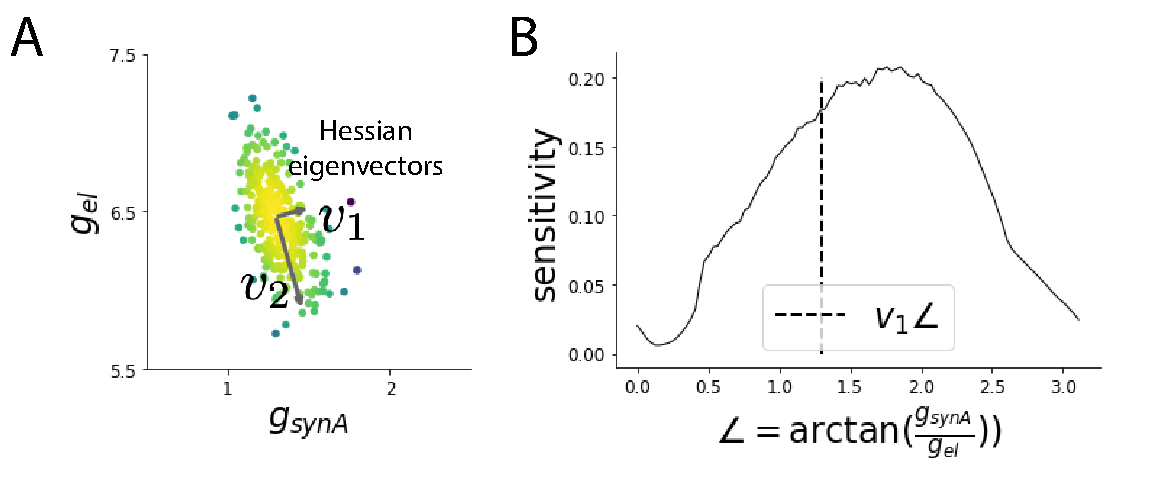
\includegraphics[scale=0.7]{figs/figS1/figS1.pdf}
\end{center}
Fig. S1: A. DSN distribution of STG model parameters producing network syncing.  B. Sensitivity of the system with respect to network syncing along all dimensions of parameter space away from the mode.
\end{figure}

\begin{figure}
\begin{center}
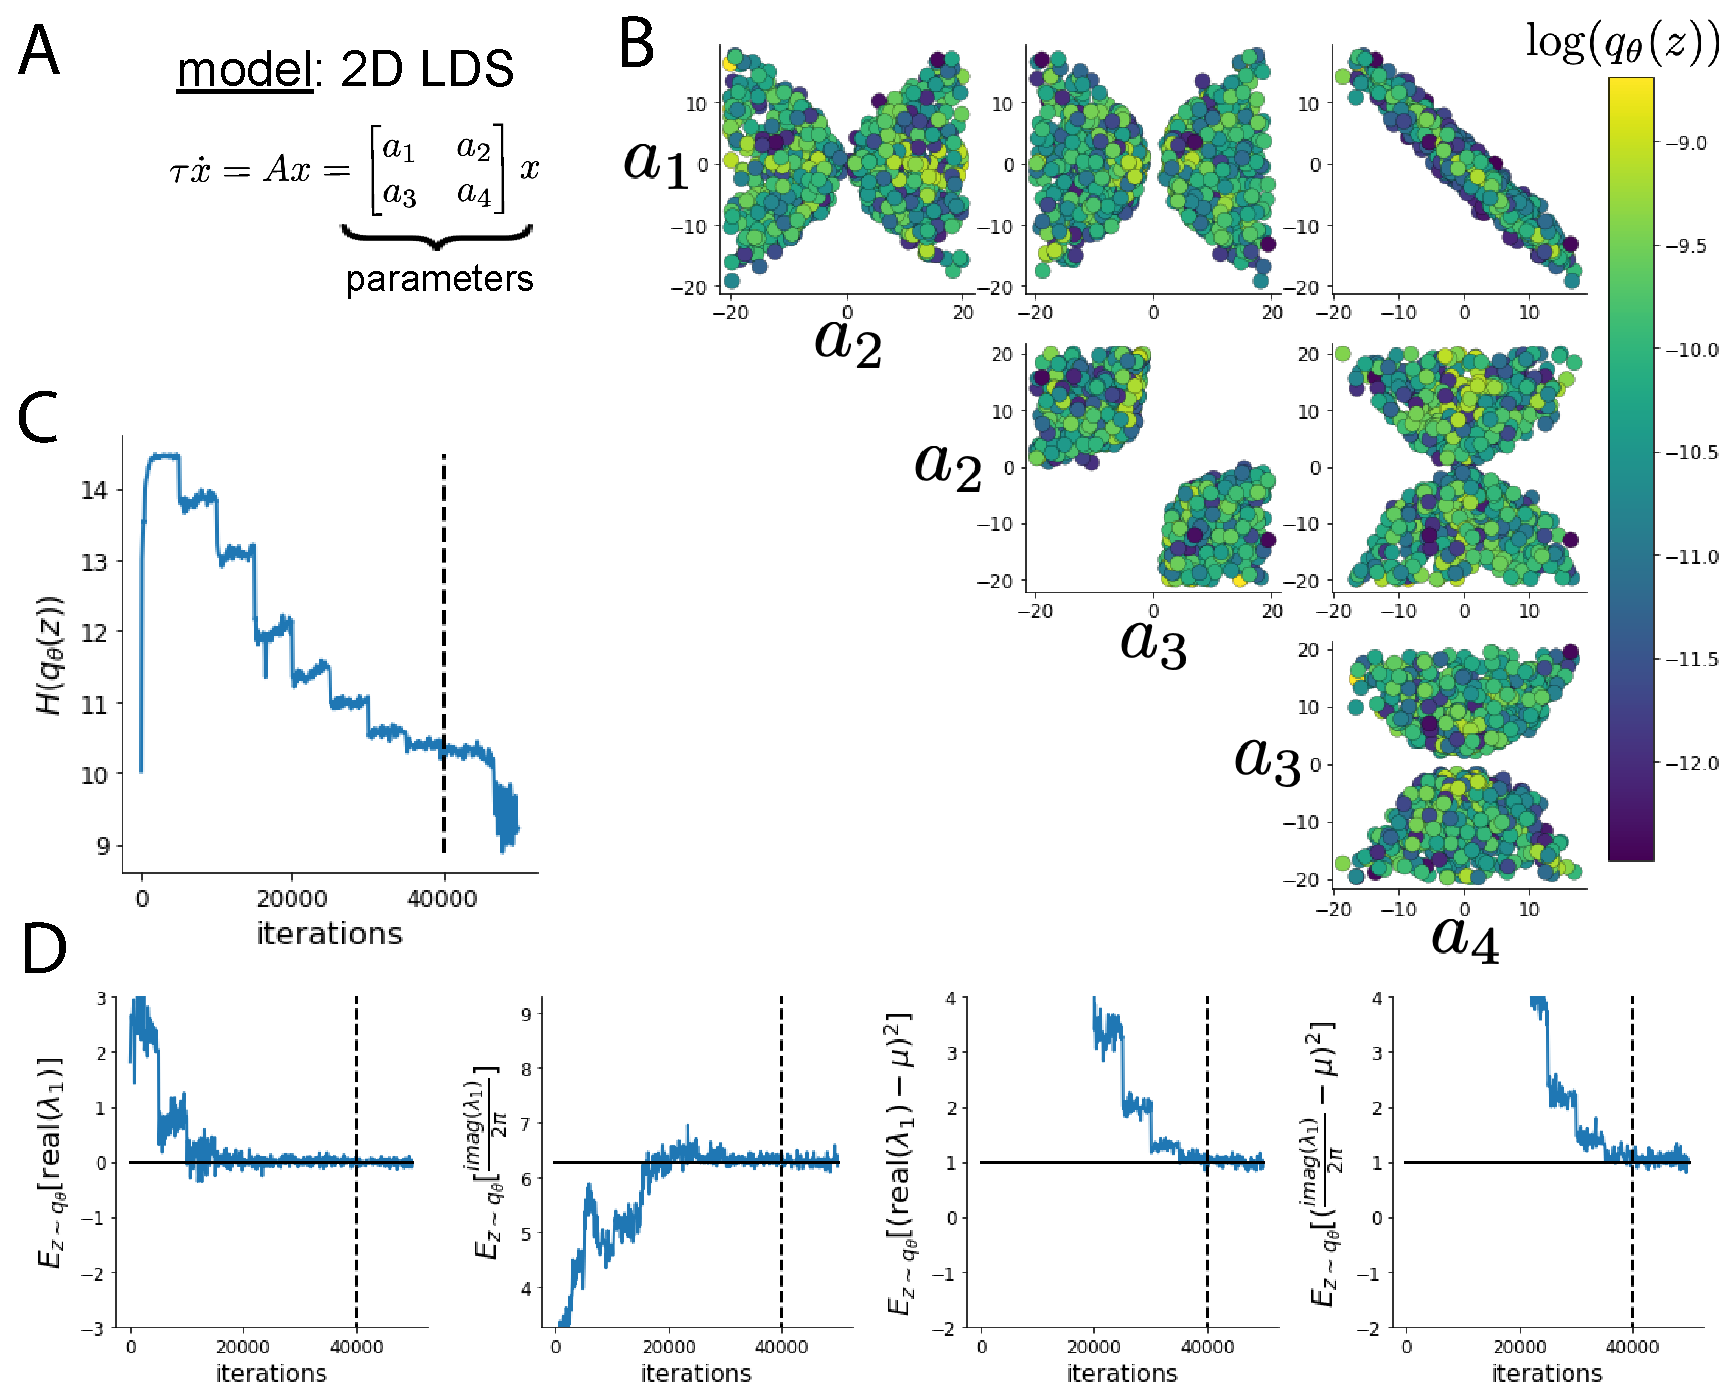
\includegraphics[scale=0.5]{figs/figS2/figS2.pdf}
\end{center}
Fig. S2: A. Two-dimensional linear dynamical system model, where real entries of the dynamics matrix $A$ are the parameters.  B. The DSN distribution for a 2D LDS with $\tau=1$ that produces an average of 1Hz oscillations with some small amount of variance.  C. Entropy throughout the optimization.  At the beginning of each augmented lagrangian epoch (5,000 iterations), the entropy dips due to the shifted optimization manifold where emergent property constraint satisfaction is increasingly weighted.  D. Emergent property moments throughout optimization.  At the beginning of each augmented lagrangian epoch, the emergent property moments move closer to their constraints.
\end{figure}


\begin{figure}
\begin{center}
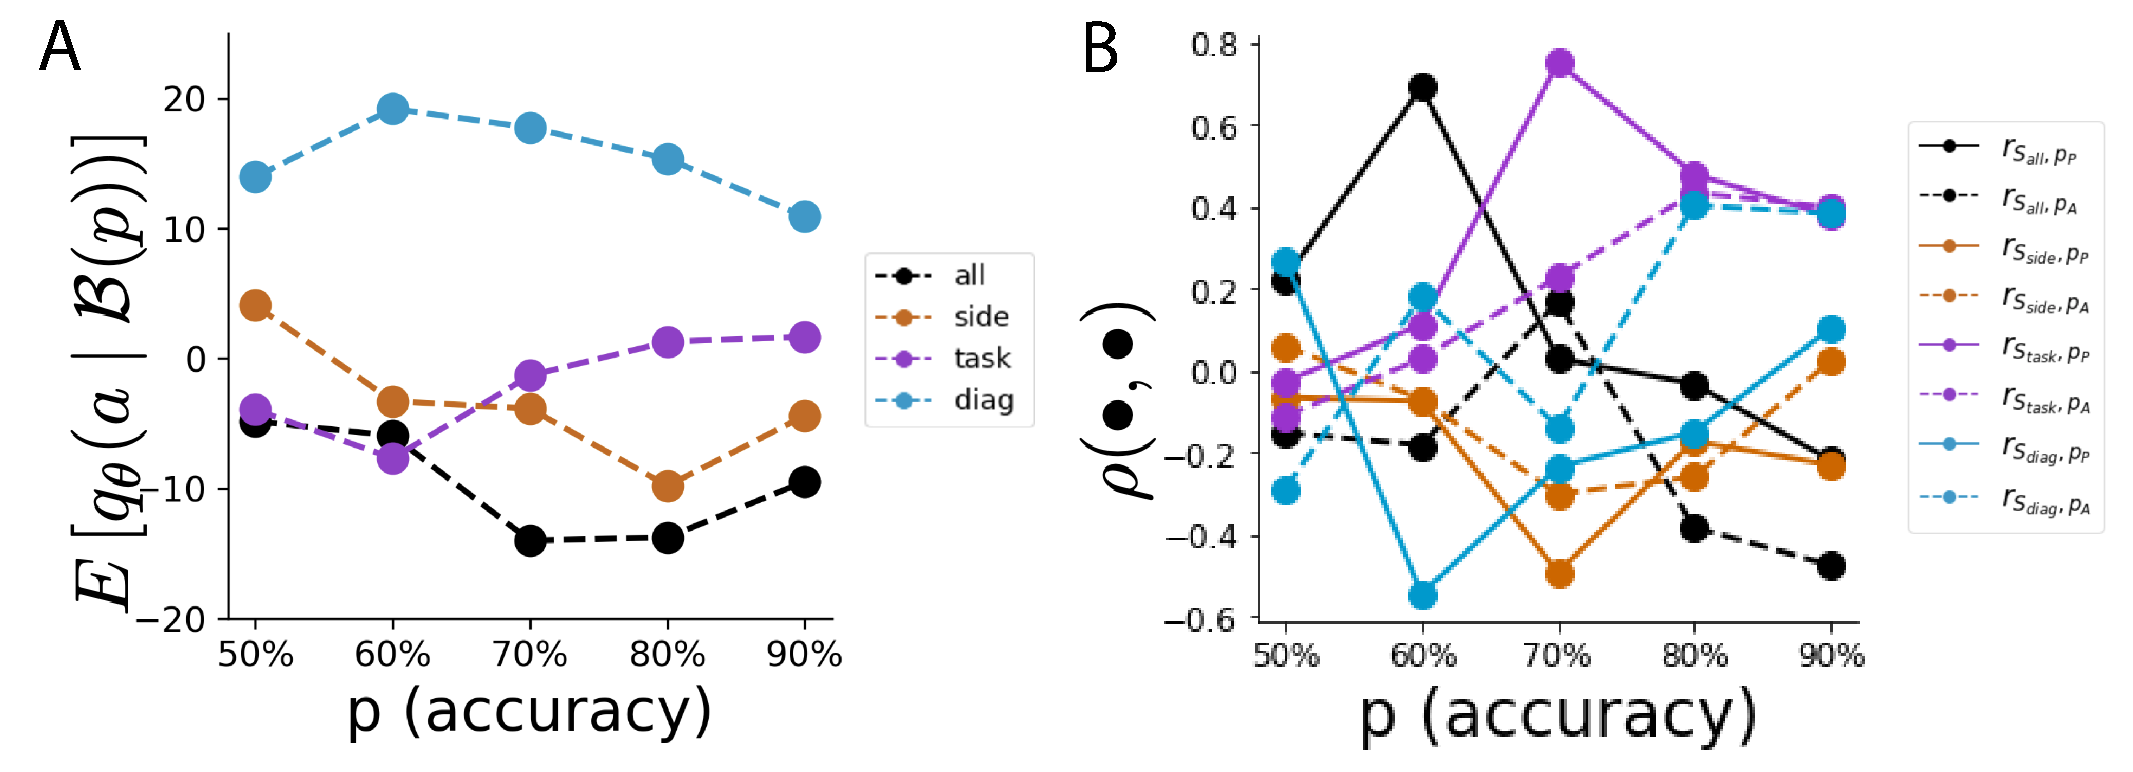
\includegraphics[scale=0.5]{figs/figS3/figS3.pdf}
\end{center}
Fig. S3: A. The mean Schur eigenvalues of each EPI posterior. B. For each EPI posterior, we measured the correlation between rapid switching accuracy for a given condition and the Schur eigenvalues.
\end{figure}

\begin{figure}
\begin{center}
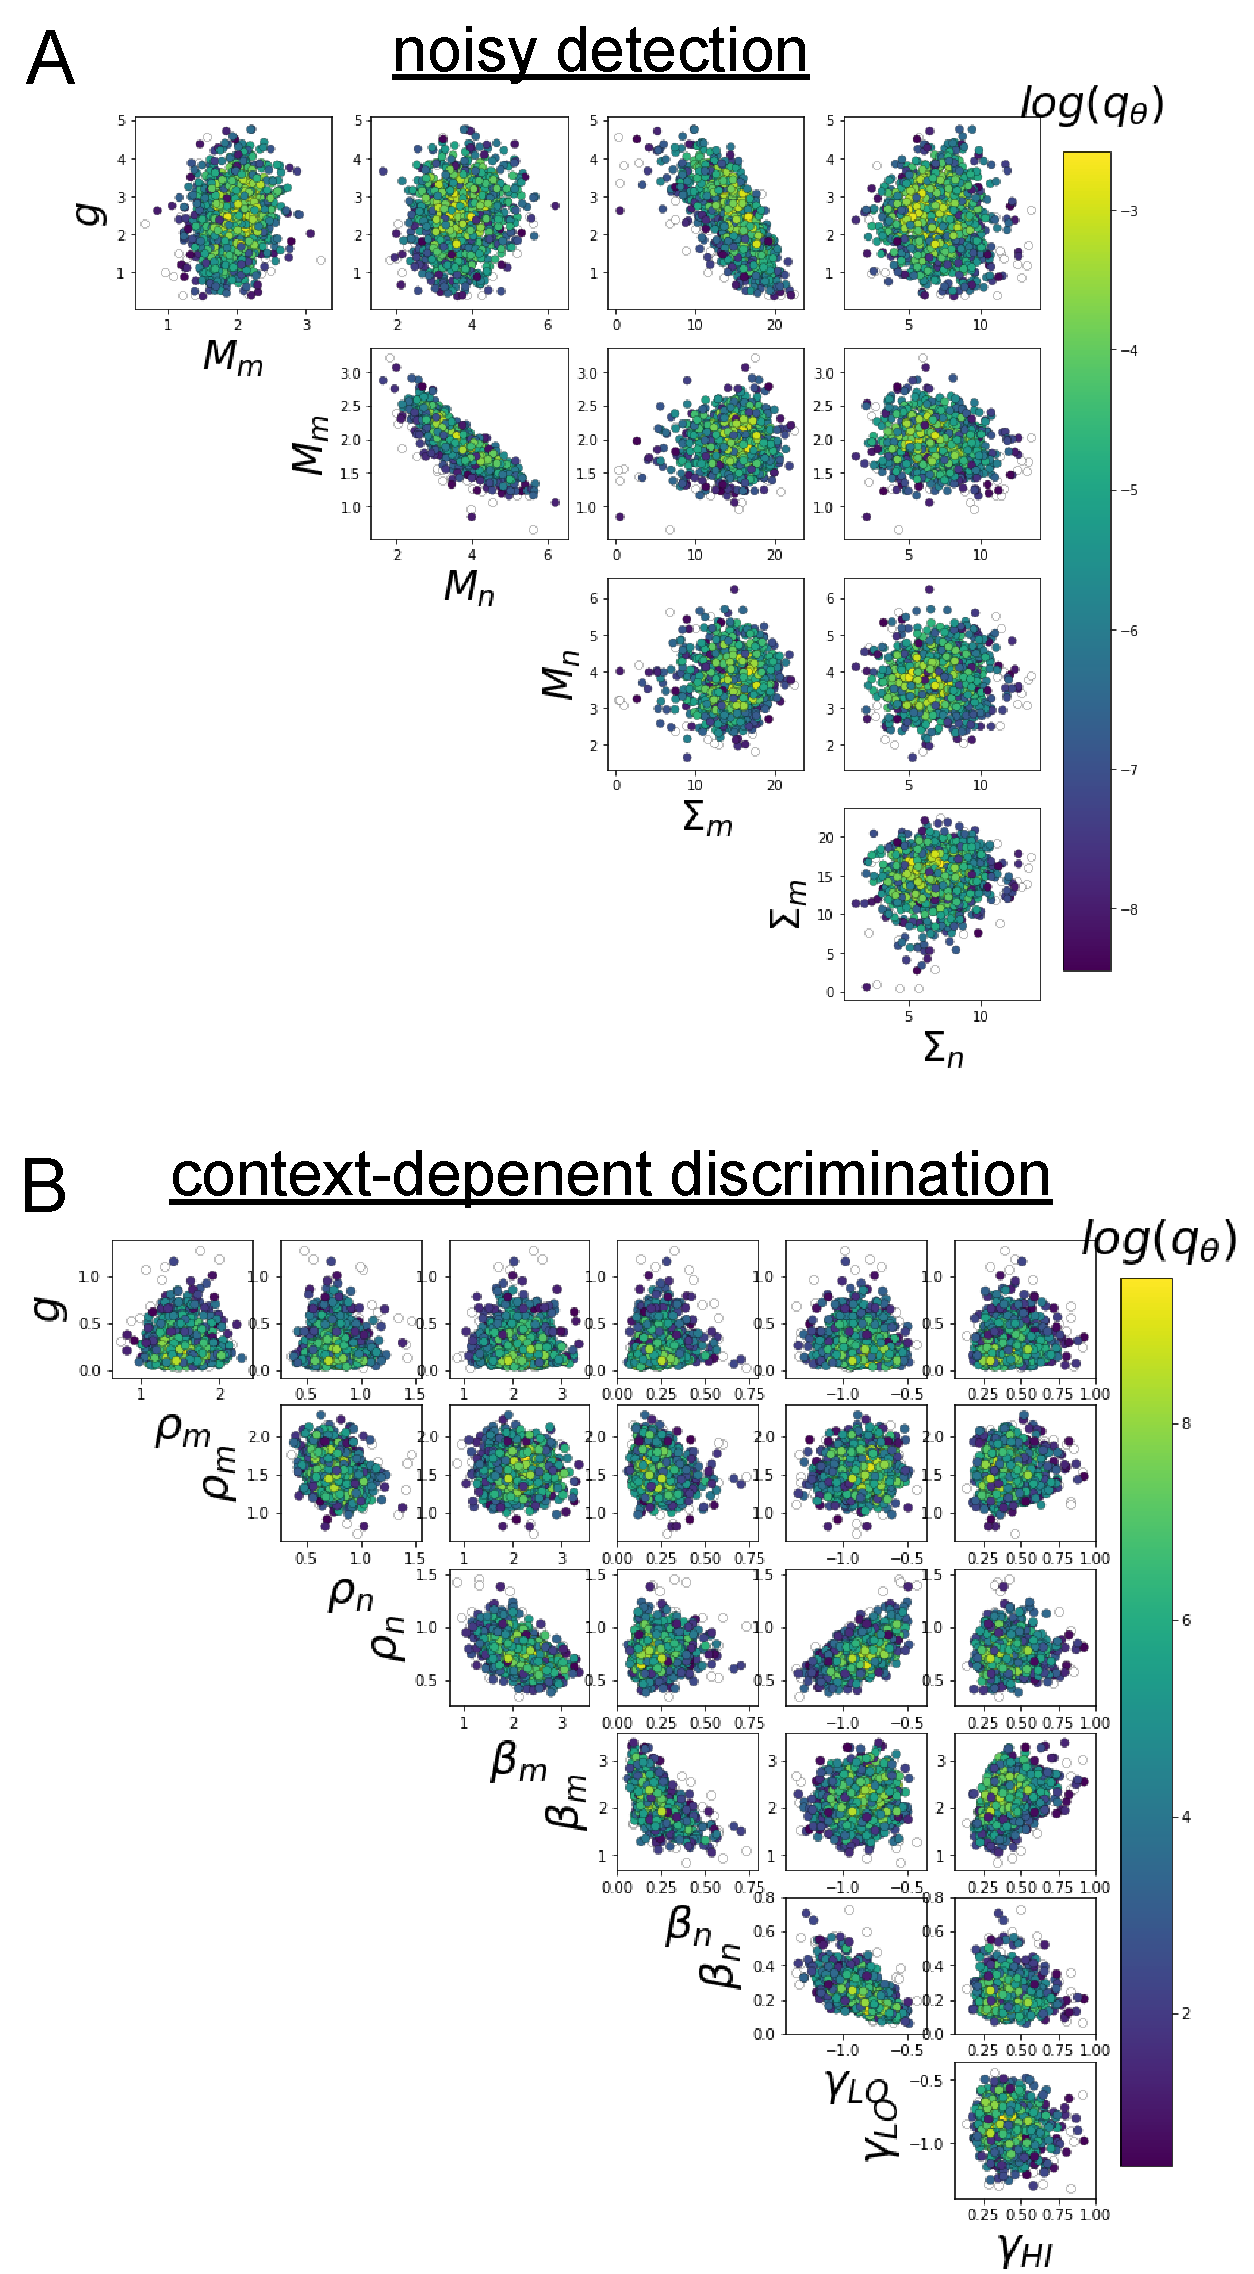
\includegraphics[scale=0.5]{figs/figS4/figS4.pdf}
\end{center}
Fig. S4: A. EPI for rank-1 networks doing discrimination. B. EPI for rank-2 networks doing context-dependent discrimination.
\end{figure}
\end{document}


